%This file is just a wrapper. Please, edit the files for your chapter in chapters/chapter1/.
\documentclass[a4paper]{report}

%%%% INCLUDE PACKAGES %%%%

\usepackage{amssymb}
\usepackage{amsmath}
\usepackage{amsthm}
\usepackage{physics}
\usepackage{geometry}
\usepackage{graphicx}
\usepackage{xcolor}
\usepackage{subfigure}
\usepackage{makeidx}
\usepackage{multicol}
\usepackage{hyperref}
\usepackage{tikz-feynman}
\usepackage{tcolorbox}
\usepackage{epigraph}
\usepackage[rightcaption]{sidecap}
\usepackage{minitoc}% for TOCs at the begining of each chapter

%%%% END PACKAGES %%%%


\frenchspacing
\renewcommand\sidecaptionsep{0.1cm}
\tolerance=50000
\makeindex
\theoremstyle{plain}
\newtheorem{theorem}{Theorem}[chapter]
\newtheorem{exercise}{Exercise}[chapter]
\newtheorem{example}{Example}
\newtheorem{definition}{Definition}[chapter]
\newtheorem{proposition}{Proposition}[chapter]
\newtheorem{corollary}{Corollary}[chapter]

\theoremstyle{remark}
\newtheorem{remark}{Remark}[chapter]

\definecolor{titlepagecolor}{cmyk}{1,.60,0,.40}
\definecolor{namecolor}{cmyk}{1,.50,0,.10} 



\hbadness=99999
\newcommand{\sn}{\mathcal{N}}
\newcommand{\hilspace}{\mathcal{H}}
\renewcommand{\baselinestretch}{1.15}


%%%%%%%%%%%%%%
% Author for each chapter %
% %%%%%%%%%%%%%%

\usepackage{lipsum}
\usepackage{suffix}

\newcommand\chapterauthor[1]{\authortoc{#1}\printchapterauthor{#1}}
\WithSuffix\newcommand\chapterauthor*[1]{\printchapterauthor{#1}}

\makeatletter
\newcommand{\printchapterauthor}[1]{%
    {\parindent0pt\vspace*{-25pt}%
        \linespread{1.1}\large\scshape#1%
          \par\nobreak\vspace*{35pt}}
            \@afterheading%
          }
          \newcommand{\authortoc}[1]{%
              \addtocontents{toc}{\vskip-10pt}%
                \addtocontents{toc}{%
                      \protect\contentsline{chapter}%
                          {\hskip1.3em\mdseries\scshape\protect\scriptsize#1}{}{}}
                            \addtocontents{toc}{\vskip5pt}%
                          }
                        \makeatother





\begin{document}


%%%% TITLE PAGE %%%%%%%%%%%%%%
\begin{titlepage}
  \newgeometry{left=7.5cm} %defines the geometry for the titlepage
  \pagecolor{titlepagecolor}
  \noindent
  
\includegraphics[width=2cm]{logo.jpg}\\[-1em]
  \color{white}
  \makebox[0pt][l]{\rule{1.3\textwidth}{1pt}}
  \par
  \noindent
  \textbf{\textsf{Sofia University}}
  \textcolor{namecolor}{\textsf{Faculty of Physics}}
  \vfill
  \noindent
  {\huge \textsf{My Journey Through Theoretical Physics}}
  \vskip\baselineskip
  \noindent
  \textsf{IVO ILIEV}
\end{titlepage}
\restoregeometry % restores the geometry
\nopagecolor% Use this to restore the color pages to white
%%%% END TITLE PAGE %%%%


%%%%%%% INCLUDE CONTENT FILES %%%%%%%%%%%
\cleardoublepage
\thispagestyle{empty}
\vspace*{\stretch{1}}
\begin{center}
\Large\itshape
To my friends,\\
my familly, my teachers and collegues.\\
Also, to Mister T\\
I pitty the fool
\end{center}
\vspace{\stretch{2}}

\cleardoublepage
\setcounter{page}{8} %previous pages will be reserved for frontmatter to be added in later.

\doparttoc
\dominitoc

\tableofcontents
\chapter*{Foreword}
\Large
\textit{"It is so shocking to find out how many people do not believe that they can learn, and how many more believe learning to be difficult."}
\begin{flushright}
Frank Herbert, Dune
\end{flushright}
\normalsize
%\vadjust{\vfill\pagebreak}



\chapter*{Preface}
The idea behind this book is to systematically put a lot of knowledge from different fields in the same place. It is envisioned to serve a purpose of an index book, a glossary introduction to modern physics. The depth may be lacking in some respects but the core idea is to have a background knowledge of many approaches and frameworks.


 % preface needs work
%%%\twocolumn
\chapter*{Contributors}

\begin{multicols}{2}
\contributor{Some Person}{Nobody Uni}{Butth Ole, Germany}

\contributor{Other Guy}{Institute of nothing}{Butth Ole, Germany}



\end{multicols}
 %this is for contributors

\mainmatter

\part{Physics}
%\chapterauthor{Second Author}{Second Author Affiliation}
\chapter{General Relativity}
\chapterauthor{Ivo Iliev\\Sofia University}
\adjustmtc
\minitoc
\section{Anti De Sitter Space (AdS)}
$AdS_n$ is an $n$-dimensional solution for the theory of gravitation with Einstein-Hilbert action with negative cosmological constant $\Lambda$, i.e. the theory described by the following Lagrangian density:
\begin{equation}
\mathcal{L} = \frac{1}{16\pi G_{(n)}}(R-2\Lambda),
\end{equation}
where $G_{(n)}$ is the gravitational constant in $n$-dimensional spacetime. Therefore, it's a solution of the Einstein field equations:
\begin{equation}
G_{\mu\nu} + \Lambda g_{\mu\nu} = 0,
\end{equation}
where $G_{\mu\nu}$ is the Einstein tensor and $g_{\mu\nu}$ is the metric of the spacetime. Introducing the radius $\alpha$ as 
\begin{equation}
\Lambda = \frac{-(n-1)(n-2)}{2\alpha^2}
\end{equation}
this solution can be immersed in a $n+1$ dimensional spacetime with signature $(-,-,+,\cdots,+)$ by the following constraint:
\begin{equation}
-X^2_1 - X^2_2 + \sum_{i=3}^{n+1}X_i^2 = -\alpha^2
\end{equation}
dadadasd

\chapterauthor{Ivo Iliev}{Sofia University}
%\chapterauthor{Second Author}{Second Author Affiliation}
\chapter{Quantum Field Theory}

\section{Sample Section}
Sample text

%%%\begin{table}
%%%    \tabletitle{Examples for illustrating attacks}
%%%    \begin{tabular}{|c|c|c|c|}
%%%        \hline
%%%        \textbf{Job} & \textbf{Sex} & \textbf{Age} & \textbf{Disease} \\
%%%        \hline
%%%        Engineer & Male & 35 & Hepatitis \\
%%%        Engineer & Male & 38 & Hepatitis \\
%%%        Lawyer & Male & 38 & HIV \\
%%%        Writer & Female & 30 & Flu \\
%%%        Writer & Female & 30 & HIV \\
%%%        Dancer & Female & 30 & HIV \\
%%%        Dancer & Female & 30 & HIV \\
%%%        \hline
%%%    \end{tabular}
%%%    \label{table:rawpatient}
%%%\end{table}

%\section{Glossary}
%\begin{Glossary}

%\end{Glossary}


%\chapterauthor{Second Author}{Second Author Affiliation}`
\chapter{Supersymmetry}
\chapterauthor{Ivo Iliev\\Sofia University}
\adjustmtc
\minitoc
\section{Supermultiplets}

\begin{definition}[Supermultiplet]
  Representations of the supersymmetric algebra (superalgebra) are called
  supermultiplets.
\end{definition}

Indeed, these representations can be thought of as multiplets where we assemble
together several different representations of the Lorentz algebra, since the
latter is a subalgebra of the superalgebra.

\subsection{Massless supermultiplets}
If $P^2=0$, then we can take $P_\mu$ to a canonical form by applying boost and
rotations until it reads

\begin{equation}
  \sigma^{\mu}_{\alpha\dot{\alpha}}P_\mu = \left(\sigma^0+\sigma^3\right)E = 
  \begin{bmatrix}
    0 & 0\\
    0 & 2E
  \end{bmatrix}
\end{equation}

The supersymmetric algebra becomes,
\begin{equation}
  \begin{bmatrix}
    \{Q_1,\bar{Q}_{\dot{1}}\} & \{Q_1,\bar{Q}_{\dot{2}}\} \\

    \{Q_2,\bar{Q}_{\dot{1}}\} & \{Q_2,\bar{Q}_{\dot{2}}\} \\

  \end{bmatrix}
  =
  \begin{bmatrix}
    0 & 0\\
    0 & 4E
  \end{bmatrix}
\end{equation}
intended as acting on the states of the multiplet we are looking for. In
particular,
\begin{equation}
\{Q_1, \bar{Q}_{\dot{1}}\} = 0
\end{equation}
which implies that 
\begin{equation}
  ||Q_1|\omega\rangle||^2 = 0 = ||\bar{Q}_{\dot{1}}|\omega\rangle||^2
\end{equation}
and thus

\begin{equation}
  Q_1|\omega\rangle = 0 = \bar{Q}_{\dot{1}}|\omega\rangle.
\end{equation}
This means that as operators $Q_1$ and $\bar{Q}_{\dot{1}}$ annihilate the
multiplet. 
\par The only non-trivial anticommutation relation that is left is:
\begin{equation}
  \{Q_2,\bar{Q}_{\dot{2}}\} = 1
\end{equation}
If we call
\begin{equation}
  \alpha = \frac{1}{2\sqrt{E}}Q_2,\quad \alpha^\dagger
  = \frac{1}{2E}\bar{Q}_{\dot{2}}
\end{equation}
then the anticommutation relation that is left is:
\begin{equation}
  \{\alpha,\alpha^\dagger\} = 1
\end{equation}
with $\{\alpha,\alpha\} = 0$.

We can build the representation starting from a state $|\lambda\rangle$ such
that
\begin{equation}
  \alpha|\lambda\rangle = 0
\end{equation}
Lets suppose that it has \textit{helicity} $\lambda$:
\begin{equation}
  M_{12}\lambda \equiv J_3|\lambda\rangle = \lambda|\lambda\rangle.
\end{equation}
It is easy to compute the helicity of $\alpha^{\dagger}|\lambda\rangle$:
\begin{equation}
  M_{12} \bar{Q}_{\dot{2}}|\lambda\rangle
  = \left(\bar{Q}_{\dot{2}}M_{12}+\frac{1}{2}\bar{Q}_{\dot{2}}\right)|\lambda\rangle
  = (\lambda+\frac{1}{2}\bar{Q}_{\dot{2}})|\lambda\rangle 
\end{equation}
In the last line, we have used the fact that
$\left[M_{12},\bar{Q}_{\dot{2}}\right]=\frac{1}{2}\bar{Q}_{\dot{2}}$. Thus we
found out that
\begin{equation}
  \alpha^\dagger|\lambda\rangle  = |\lambda+ \frac{1}{2}\rangle 
\end{equation}
Since $(\alpha^\dagger)^2 = 0$, this stops here. Hence we have
\begin{equation}
  \alpha^\dagger|\lambda+\frac{1}{2}\rangle = 0.
\end{equation}
\par
Massless multiplets are thus composed of one boson and one fermion. Since
physical particles must come in CPT conjugate representation (or, there are no
spin-$\frac{1}{2}$ one dimensional representations of the massless little group
of the Lorentz group), one must add the CPT conjugate multiplet where
helicities are flipped.
\begin{example}[Examples of massless supermultiplets]
  \mbox{}
  \begin{itemize}
    \item The \textit{scalar} multiplet is obtained by setting $\lambda =0$.
      Then we have 
      \begin{equation}
        \alpha^\dagger\ket{0} = \ket{\frac{1}{2}}
      \end{equation}
      The full multiplet is composed of two states with $\lambda = 0 $ and
      a doublet with $\lambda = \pm\frac{1}{2}$. These are the degrees of
      freedom of a complex scalar and a Weyl (chiral) fermion.
    \item The \textit{vector} multiplet is obtained starting from a $\lambda
      = \frac{1}{2}$ state. We get
      \begin{equation}
        \alpha^\dagger\ket{\frac{1}{2}} = \ket{1}.
      \end{equation}
      To this we add the CPT conjugate multiplet, to obtain two pairs of
      states, one with $\lambda = \pm\frac{1}{2}$ and the other with $\lambda
      = \pm 1$. These are the degrees of freedom of a Weyl fermion and of
      a massless vector. The latter is usually interpreted as a gauge boson.
    \item Another multiplet is obtained starting from $\lambda = \frac{3}{2}$:
      \begin{equation}
        \alpha^\dagger\ket{\frac{3}{2}} = \ket{2}.
      \end{equation}
      Adding the CPT conjugate, one has a pair of bosonic degrees of freedom
      with $\lambda = \pm 2$, which we interpret as the \textit{graviton}, and
      a pair of fermionic degrees of freedom with $\lambda =\pm\frac{3}{2}$,
      which correspond to a massless spin-$\frac{3}{2}$ Rarita-Schwinger field,
      also called the \textit{gravition}, since it is the SUSY partner of the
      graviton, as was just shown.
  \end{itemize}
\end{example}
\subsection{Supermultiplets of extended supersymmetry}
Very briefly we will mention that having extended SUSY, the massless
supermultiplets are longer. Let's take the algebra to be:
\begin{equation}
  \{Q_\alpha^I,\bar{Q}_{\dot{\alpha}}^J\} = 2\sigma_{\alpha\dot{\alpha}}^\mu
  P_\mu\delta^{IJ},
\end{equation}
where for simplicity we suppose that $Z^{IJ}=0$ for these states. For massless
states, $P_\mu = (E,0,0,E)$ and therefore as before we have that
\begin{equation}
  \{Q_1^I,\bar{Q}_{\dot{1}}^J\} = 0,
\end{equation}
which implies the (operator) equations $Q_1^I=0$ and $\bar{Q}_{\dot{1}}^I=0$,
for $I=1,\cdots,\sn$. The non-trivial relations are then:
\begin{equation}
\{Q_2^I, \bar{Q}_{\dot{2}}^J\} = 4E\delta^{IJ}
\end{equation}
Of course we can define
\begin{equation}
  \alpha_I = \frac{1}{2\sqrt{E}}Q_2^I
\end{equation}
and obtain the canonical anticommutation relations for $\sn$ fermionic
oscillators
\begin{equation}
  \{\alpha_I,\alpha_J^\dagger\} = \delta_{IJ}
\end{equation}
\par If we now start with a state $\ket{\lambda}$ with helicity $\lambda$ which
satisfies $\alpha_I\ket{\lambda} = 0$, we build a multiplet as follows:
\begin{gather}
  \alpha_I^\dagger\ket{\lambda} = \ket{\lambda + \frac{1}{2}}_I,\nonumber\\
  \alpha_I\dagger\alpha_J\dagger\ket{\lambda} = \ket{\lambda
  + 1}_{[IJ]},\nonumber\\
  \vdots\nonumber\\
  \alpha_1^\dagger\cdots\alpha_{\sn}^\dagger\ket{\lambda}
  = \ket{\lambda+\frac{\sn}{2}}
\end{gather}
It is very important to note that there are $\sn$ states with helicity
$\lambda + \frac{1}{2}, \frac{1}{2}\sn(\sn-1)$ states with
helicity $\lambda + 1$ and so on, until we reach a single state with helicity $\lambda
+\frac{\sn}{2}$ (it is totally antisymmetric in $\sn$ indices
I). In total, the supermultiplet is composed of $2^\sn$ states, half of
them bosonic and half of them fermionic.
\par Interestingly, in this case we can now have self-CPT conjugate multiplets.
Take for example $\sn = 4$ and start from $\lambda = -1$. Then $\lambda
+ \frac{\sn}{2} = 1$ and the multiplet spans states of opposite helicities,
thus filling complete representations of the Lorenz group. Indeed, it contains
one pair of states with $\lambda\pm1$ (a vector, i.e a gauge boson), 4 pairs of
states with $\lambda=\pm\frac{1}{3}$ (4 Weyl Fermions) and 6 states with
$\lambda = 0$ (6 real scalars, or equivalently 3 complex scalars).
\par Another example is $\sn = 8$ supersymmetry. Here if we start with $\lambda
= -2$ we end up with $\lambda + \frac{\sn}{2} = 2$. Thus in this case we have
the graviton in the self-CPT conjugate multiplet, corresponding to the pair of
states with $\lambda\pm2$. In addition, we have 8 massless gravitini with
$\lambda\pm\frac{3}{2}$, 28 massless vectors with $\lambda = \pm 1$, 56
massless Weyl fermions with $\lambda = \pm\frac{1}{2}$ and finally 70 real
scalars with $\lambda = 0$. This is the content of $\sn = 8$
\textit{supergravity}, which is the only multiplet of $\sn = 8$ supersymmetry
with $|\lambda|<2$. The latter condition is necessary in order to have
consistent couplings (higher spin fields cannot be coupled in a consistent way
with gravity and lower spin fields).
\par From the theoretical standpoint, this is a very nice result, because we
have a theory where \textit{everything is determined} from symmetry alone: the
complete spectrum and all the couplings. Unfortunately, this theory is also
completely unphysical. To mention one problem, it has no room for fermions in
complex representations of the gauge group, which are present in the Standard
Model.

\subsection{Massive supermultiplets}
When $P^2=M^2>0$, by boosts and rotation $P_\mu$ can be put in the following
form
\begin{equation}
  P_\mu = (M,0,0,0)
\end{equation}
Then we have
\begin{equation}
  \sigma_{\alpha\dot{\alpha}}^\mu P_\mu = M\sigma^0 = 
  \begin{bmatrix} 
    M & 0\\
    0 & M
  \end{bmatrix}
\end{equation}
so that the superalgebra reads
\begin{equation}
  \{Q_\alpha, \bar{Q}_{\dot{\alpha}}\} = 2 M\delta_{\alpha\dot{\alpha}}
\end{equation}
Note that $[M_{12}, Q_1] = i(\sigma_{12})_1\ ^1Q_1= \frac{1}{2}Q_1$, thus it is
$Q_1$ that raises the helicity, in the same way as $\bar{Q}_{\dot{2}}$. We make
the redefinition
\begin{gather}
  \alpha_1 = \frac{1}{\sqrt{2M}}\bar{Q}_{\dot{1}},\quad \alpha_1^\dagger
  = \frac{1}{\sqrt{2M}}Q_1, \\
  \alpha_2 = \frac{1}{\sqrt{2M}}Q_2,\quad \alpha_2^\dagger
  = \frac{1}{\sqrt{2M}}\bar{Q}_{\dot{2}},
\end{gather}
so that we have the canonical anticommutation relations of two fermionic
oscillators:
\begin{equation}
  \{\alpha_a,\alpha_b^\dagger\}=\delta_{ab},\quad a,b = 1,2.
\end{equation}
\par If we start with $\alpha_a\ket{\lambda} = 0$, $M_{12}\ket{\lambda}
= \lambda\ket{\lambda}$, then we build the multiplet as:
\begin{gather}
  \alpha_1^\dagger\ket{\lambda} = \ket{\lambda + \frac{1}{2}}_1,\\
  \alpha_2^\dagger\ket{\lambda} = \ket{\lambda+\frac{1}{2}}_2,\\
  \alpha_1^\dagger\alpha_2^\dagger\ket{\lambda} = \ket{\lambda+1}.
\end{gather}
There are 4 states now (compared to the 2 in the massless case), two bosons and
two fermions. 
\begin{example}[Examples of massive supermultiplets]
  \mbox{}
  \begin{itemize}
    \item In the case of the \textit{massive scalar multiplet}, we start from
      $\lambda =  -\frac{1}{2}$ and obtain two states with $\lambda=0$ and one
      state with $\lambda=\frac{1}{2}$. These are the degrees of freedom of one
      massive complex scalar and one massive Weyl fermion. Note that the latter
      might not be familiar. Indeed, one cannot write the usual Dirac mass term
      for a Weyl fermion. Instead, one can write what is called a Majorana mass
      term:
      \begin{equation}
        \mathcal{L}\supset m\epsilon^{\alpha\beta}\psi_\alpha\psi_\beta + h.c.
      \end{equation}
      Note that the total degrees of freedom of a massless scalar multiplet is
      the same as that of a massive one.
    \item For a \textit{massive vector multiplet}, start from $\lambda = 0$ to
      obtain 2 states with $\lambda = \frac{1}{2}$ and one state with $\lambda
      = 1$. To this we add the CPT conjugate multiplet so that in the end we
      have one pair with $\lambda = \pm1$, two pairs with
      $\lambda=\pm\frac{1}{2}$ and two states with $\lambda = 0$. According to
      the massive little group, this corresponds to 1 massive vector (with
      $\lambda = \pm1,0)$, 1 real scalar and 1 massive Dirac fermion. Note
      however that the content in degrees of freedom is the same as that of one
      massless vector multiplet together with one massless scalar multiplet.
      This hints that the consistent way to treat massive vectors in
      a supersymmetric field theory will be through a SUSY version of the
      Brout-Englert-Higgs mechanism.
    \end{itemize}

  \end{example}
\section{General}
\begin{definition}[R-symmetry]
In supersymmetric theories, an R-symmetry is the symmetry transforming
different supercharges into each other. In the simplest case of the $\sn=1$
supersymmetry, such R-symmetry is isomorphic to a global $U(1)$ group or its discrete subgroup. For extended supersymmetry theories, the R-symmetry group becomes a global non-abelian group.  
\end{definition}

\begin{remark}
In the case of the discrete subgroup $\mathbb{Z}_2$, the R-symmetry is called \textit{R-parity}
\end{remark}

\begin{definition}[Extended supersymmetry]
In supersymmetric theories, when $\sn>1$ the algebra is said to have
\textit{extended supersymmetry}.
\end{definition}

\section{Bogomol'nyi-Prasad-Sommerfield (BPS) states}
\begin{definition}[BPS state]
A massive representation of an extended supersymmetry algebra that has mass
equal to the supersymmetry central charge $Z$ is called an \textit{BPS} state.
\end{definition}

Quantum mechanically speaking, if the supersymmetry remains unbroken, exact
solutions to the modulus of $Z$ exist. Their importance arises as the
multiplets shorten for generic representations, with stability and mass formula
exact.

\begin{example}[$d=4$,$\sn=2$]
The generators for the odd part of the superalgebra have relations:
\begin{gather}
  \{Q_\alpha^A,\bar{Q}_{\dot{\beta}B}\} = 2\sigma^m_{\alpha\dot{\beta}}P_m\delta^A_B \\
  \{Q_\alpha^A,Q_{\beta B}\} = 2\epsilon_{\alpha\beta}\epsilon^{AB}\bar{Z}\\
  \{\bar{Q}_{\dot{\alpha}A},\bar{Q}_{\dot{\beta}B}\}
  = -2\epsilon_{\dot{\alpha}\dot{\beta}}\epsilon_{AB}Z,
\end{gather}
where $\alpha\dot{\beta}$ are the Lorentz group indices and $A,B$ are the
$R$-symmerty indices.
If we take linear combinations of the above generators as follows:
\begin{gather}
  R_\alpha^A = \xi^{-1}Q_\alpha^A
  + \xi\sigma^0_{\alpha\dot{\beta}}\bar{Q}^{\dot{\beta}B}\\
  T_\alpha^A = \xi^{-1}Q_\alpha^A - \xi\sigma^0_{\alpha\dot{\beta}}\bar{Q}^{\dot{\beta}B}
\end{gather}
and consider a state $\psi$ which has momentum $(M,0,0,0)$, we have:
\begin{equation}
  \left(R_1^1+(R_1^1)^\dagger\right)^2\psi = 4(M+Re(Z\xi^2))\psi,
\end{equation}
but because this is the square of a Hermitian operator, the right hand side
coefficient must be positive for all $\xi$. In particular, the strongest result from this is
\begin{equation}
  M\geq|Z|
\end{equation}
\end{example}
\section{Supersymmetric theories on curved manifolds}
\textit{Remark:} Supersymmetric theories may be defined only on backgrounds admitting solutions to certain Killing spinor equations,
\begin{align}
\left(\nabla_\mu-iA_\mu\right)\zeta + iV_\mu\zeta + iV^\nu\sigma_{\mu\nu}\zeta = 0\\
\left(\nabla_\mu+iA_\mu\right)\tilde{\zeta} - iV_\mu\tilde{\zeta} -  iV^\nu\tilde{\sigma}_{\mu\nu}\tilde{\zeta} = 0
\end{align}
which in four dimensions and Euclidean signature are
equivalent to the requirement that the manifold is complex and the metric Hermitian.

\section{Supersymmetric Chern-Simons-matter theories}

In this section we will introduce the basic building blocks of supersymmetric
Chern-Simons-matter theories. We will work in Euclidean space, and we will put
the theories on the three-sphere, since we are eventually interested in
computing the free energy of the gauge theory in this curved space. 
\subsection{Conventions}
In Euclidean space, the fermions $\psi$ and $\bar{\psi}$ are independent and 
they transform and they transform in the same representation of the Lorentz
group. Their index structure is:
\begin{equation}
  \psi^\alpha, \quad\bar{\psi}^\alpha .
\end{equation}
We will take $\gamma_\mu$ to be the Pauli matrices, which are hermitian, and
\begin{equation}
  \gamma_{\mu\nu} = \frac{1}{2}\left[\gamma_\mu,\gamma_nu\right]
= i\epsilon_{\mu\nu\rho}\gamma^{\rho}
\end{equation}
We introduce the usual symplectic product through the antisymmetric matrix
\begin{equation}
  C_{\alpha\beta} = 
  \begin{pmatrix}
        0 & C\\
        -C & 0
  \end{pmatrix}.
\end{equation}
We set $C=-1$ and denote the matrix by $\epsilon_{\alpha\beta}$. The product
is
\begin{equation}
  \bar{\epsilon}\lambda = \bar{\epsilon}^\alpha
  C_{\alpha\beta}\lambda^\beta .
\end{equation}
Notice that
\begin{equation}
  \bar{\epsilon}\gamma^\mu\lambda = \bar{\epsilon}^\beta
  C_{\beta\gamma}(\gamma^\mu)^\gamma_\alpha\lambda^\alpha .
\end{equation}
It is easy to check that
\begin{equation}
\bar{\epsilon}\lambda = \lambda\bar{\epsilon},\quad
\bar{\epsilon}\gamma^\mu\lambda = -\lambda\gamma^\mu\bar{\epsilon},
\end{equation}
and in particular
\begin{equation}
  (\gamma^\mu\bar{\epsilon})\lambda = -\bar{\epsilon}\gamma^\mu\lambda .
\end{equation}
We also have the following Fierz identities
\begin{equation}
  \bar{\epsilon}(\epsilon\psi) + \epsilon(\bar{\epsilon}\psi)
  + (\bar{\epsilon}\epsilon)\psi = 0
\end{equation}
and
\begin{equation}
  \epsilon(\bar{\epsilon}\psi) + 2(\bar{\epsilon}\epsilon)\psi
  + (\bar{\epsilon}\gamma_\mu\psi)\gamma^\mu\epsilon = 0.
\end{equation}
\subsection{Vector multiplet and supersymmetric Chern-Simons theory}
  We first start with theories based on vector multiplets. The three
  dimensional Euclidean $\mathcal{N}=2$ vector superfield $V$ has the following
  content
  \begin{equation}
    V: \quad A_\mu,\sigma,\lambda,\bar{\lambda}, D,
  \end{equation}
  where $A_\mu$ is a gauge field, $\sigma$ is an auxiliary scalar field,
  $\lambda,\bar{\lambda}$ twi-component complex Dirac spinors, and $D$ is an 
  auxiliary scalar. This is just the dimensional reduction of the
  $\mathcal{N}=1$ vector multiplet in 4 dimensions, and $\sigma$ is the
  reduction of the fourth component of $A_\mu$. All fields are valued in
  the Lie algebra $\mathfrak{g}$ of the gauge group $G$. For $G=U(N)$ our 
  convention is that $\mathfrak{g}$ are Hermitian matrices. It follows
  that the gauge covariant derivative is given by
  \begin{equation}
    \partial_\mu + i\left[A_\mu,.\;\right]
  \end{equation}
  while the gauge field strength is
  \begin{equation}
    F_{\mu\nu} = \partial_\mu A_\nu - \partial_\nu A_\mu
    + i\left[A_\mu,A_\nu\right].
  \end{equation}
The transformations of the fields are generated by two independent complex 
structures $\epsilon$, $\bar{\epsilon}$. They are given by,
\begin{align}
  \delta A_\mu &= \frac{i}{2}(\bar{\epsilon}\gamma_\mu\lambda
  - \bar{\lambda}\gamma_\mu\epsilon),\nonumber\\
  \delta\sigma &= \frac{1}{2}({\bar{\epsilon}}\lambda
  - \bar{{\lambda}}\epsilon),\nonumber\\
  \delta\lambda &= -\frac{1}{2}\gamma^{\mu\nu}\epsilon F_{\mu\nu} - D\epsilon
  + i\gamma^\mu\epsilon D_\mu\sigma + \frac{2i}{3}\sigma\gamma^\mu
  D_\mu\epsilon,\nonumber\\
  \delta\bar{\lambda} &= - \frac{1}{2}\gamma^{\mu\nu}F_{\mu\nu} + D\bar{\epsilon}
  - i\gamma^\mu\bar{\epsilon}D_\mu\sigma
  - \frac{2i}{3}\sigma\gamma^{\mu}D_\mu\bar{\epsilon},\nonumber\\
  \delta D &= -\frac{i}{2}\bar{\epsilon}\gamma^\mu D_\mu\lambda
  - \frac{i}{2}D_\mu\bar{\lambda}\gamma^\mu\epsilon
  + \frac{i}{2}\left[\bar{\epsilon}\lambda,\sigma\right]
  + \frac{i}{2}\left[\bar{\lambda}\epsilon, \sigma\right]
  - \frac{i}{6}(D_\mu\bar{\epsilon}\gamma^\mu\lambda
  + \bar{\lambda}\gamma^{\mu}D_\mu\epsilon),
\end{align}
and we split naturally
\begin{equation}
\delta = \delta_\epsilon + \delta_{\bar\epsilon}.
\end{equation}
Here we follow the conventions of \cite{Hama11}, be we change the sign of the gauge
connection: $A_\mu\rightarrow - A_\mu$. The derivative $D_\mu$ is covariant
with respect to both the gauge field and the spin connection. On all the
fields, except $D$, the commutator
$\left[\delta_{\epsilon},\delta_{\bar{\epsilon}}\right]$ becomes a sum
of translation, gauge transformation, Lorentz rotation, dilation and
$R$-rotation:
\begin{align}
  \left[\delta_\epsilon, \delta_{\bar{\epsilon}}\right]A_\mu
  &= iv^\nu\partial_\nu A_\mu + i\partial_\mu\nu^\nu A_\nu
  - D_\mu\Lambda,\nonumber\\
  \left[\delta_\epsilon, \delta_{\bar{\epsilon}}\right]\sigma
  &= i\nu^\mu\partial_\mu\sigma + i\left[\Lambda, \sigma\right] + \rho\sigma,
  \nonumber\\
  \left[\delta_\epsilon, \delta_{\bar{\epsilon}}\right]\lambda
  &= i\nu^\mu\partial_\mu\lambda
  + \frac{i}{4}\Theta_{\mu\nu}\gamma^{\mu\nu}\lambda + i\left[\Lambda,
  \lambda\right] + \frac{3}{2}\rho\lambda + \alpha\lambda,\nonumber\\
  \left[\delta_\epsilon, \delta_{\bar{\epsilon}}\right]\bar{\lambda}
  &= i\nu^\mu \partial_\mu\bar{\lambda}
  + \frac{i}{4}\Theta_{\mu\nu}\bar{\lambda} + i\left[\Lambda,
  \bar{\lambda}\right] + \frac{3}{2}\rho\bar{\lambda}
  - \alpha\bar{\lambda},\nonumber\\
  \left[\delta_\epsilon, \delta_{\bar{\epsilon}}\right]D &=i\nu^\mu\partial_\mu
  D + i\left[\Lambda, D\right] + 2\rho
  D + \frac{1}{3}\sigma(\bar{\epsilon}\gamma^\mu\gamma^{\nu}D_\mu D_\nu\epsilon
  -\epsilon\gamma^\mu\gamma^\nu D_\mu D_\nu\bar{\epsilon}),
\end{align}
where
\begin{align}
  \nu^\mu &= \bar{\epsilon}\gamma^\mu\epsilon,\nonumber\\
  \Theta^{\mu\nu} &= D^{[\mu}v^{\nu]}
  + \nu^\lambda\omega^{\mu\nu_\lambda},\nonumber\\
  \Lambda &= \nu^\mu i A_\mu + \sigma\bar{\epsilon}\epsilon\nonumber\\
  \rho &= \frac{i}{3}(\bar{\epsilon}\gamma^{\mu}D_\mu\epsilon + D_\mu
  \bar{\epsilon}\gamma^\mu\epsilon),\nonumber\\
  \alpha &= \frac{i}{3}(D_\mu\bar{\epsilon}\gamma^{\mu}\epsilon
  - \bar{\epsilon}\gamma^\mu D_\mu\epsilon).
\end{align}
Here, $\omega_\lambda^{\mu\nu}$ is the spin connection. As a check, let us
calculate the commutator acting on $\sigma$. We have,
\begin{align}
  \left[\delta_\epsilon, \delta_{\bar{\epsilon}}\right]\sigma
  &= \delta_\epsilon\left(\frac{1}{2}\bar{\epsilon}\lambda\right)
  - \delta_{\bar{\epsilon}}\left(-\frac{1}{2}\bar{\lambda}\epsilon\right)\nonumber\\
  &=\frac{1}{2}\bar{\epsilon}\left(-\frac{1}{2}\gamma^{\mu\nu}\epsilon
    F_{\mu\nu}
  - D\epsilon + i\gamma^\mu\epsilon D_\mu \sigma\right)
  + \frac{i}{3}\bar{\epsilon}\gamma^{\mu}(D_\mu\epsilon)\sigma\nonumber\\
  &+ \frac{1}{2}(-\frac{1}{2}\gamma^{\mu\nu}\bar{\epsilon}F_{\mu\nu}
  + D\epsilon - i\gamma^{\mu}\bar{\epsilon}D_\mu\sigma)\epsilon
  - \frac{i}{3}\gamma^\mu(D_\mu\bar{\epsilon})\epsilon\sigma\nonumber\\
  &= i\bar{\epsilon}\gamma^\mu\epsilon D_\mu\sigma + \rho\sigma.
\end{align}
In order for the supersymmetry algebra to close, the last term in the RHS of
$\left[\delta_\epsilon, \delta_{\bar{\epsilon}}\right]D$ must vanish. This is
the case if the Killing spinors satisfy:
\begin{equation}
  \gamma^\mu\gamma^\nu D_\mu D_\nu\epsilon = h\epsilon,\quad
  \gamma^\mu\gamma^\nu D_\mu D_\nu \bar{\epsilon} = h\bar{\epsilon}
  \label{eq:spinorrequirement}
\end{equation}
for some scalar function $h$. A sufficient condition for this is to simply have
\begin{equation}
  D_\mu\epsilon = \frac{i}{2r}\gamma_\mu\epsilon, \quad
  D_\mu\bar{\epsilon}=\frac{i}{2r}\gamma y_\mu\bar{\epsilon}
\end{equation}
and
\begin{equation}
  h = - \frac{9}{4r^2}
  \label{eq:equationh}
\end{equation}
where $r$ is the radius of the three-sphere. This condition is satisfied by one
of the Killing spinors on the three-sphere (the one which is constant in the
left-invariant frame). Notice that, with this choice $\rho$ vanishes.
\par The Euclidean SUSY Chern-Simons (CS) action, in flat space, is given by
\begin{align}
  S_{SCS} &= - \int d^3x \mathrm{Tr}\left(A\wedge dA + \frac{2i}{3}A^3
    - \bar{\lambda}\lambda + 2D\sigma\right)\\
    &= -\int d^3x
    \mathrm{Tr}\left(\epsilon^{\mu\nu\rho}\left(A_\mu\partial_\nu A_\rho
      + \frac{2i}{3}A_\mu A_\nu A_\rho\right)
    - \bar{\lambda}{\lambda}+2D\sigma\right).
  \end{align}

  Here $\mathrm{Tr}$ denotes the trace in the fundamental representation. The
  part of the action involving the gauge connection $A$ is the standard,
  bosonic CS action in three dimensions. This action was first considered
  from the point of view of QFT, in \cite{Deser82}, where the total action for
  a non-abelian gauge field was the sum of the standard Yang-Mills action and
  the CS action. In \cite{Witten89}, the CS action was considered by itself and shown
  to lead to a topological gauge theory.
  \par We can check that the SUSY CS action is invariant under the
  supersymmetry generated by $\delta_\epsilon$ (the proof for
  $\delta_{\bar{\epsilon}}$ is similar). The  SUSY variation of the integrand
  of the action is
  \begin{multline}
    (2\delta A_\mu\partial_\nu A_\rho + 2i\delta A_\mu A_\nu
    A_\rho)\epsilon^{\mu\nu\rho} - \bar{\lambda}\delta\lambda + 2(\delta
    D)\sigma + 2D\delta\sigma = \\-i\bar{\lambda}\gamma_\mu\epsilon\partial_\nu
    A_\rho\epsilon^{\mu\nu\rho} + \bar{\lambda}\gamma_\mu\epsilon A_\nu A_\rho
    \epsilon^{\mu\nu\rho} - \bar{\lambda}(-\frac{1}{2}\gamma^{\mu\nu}F_{\mu\nu}
    - D + i\gamma^\mu D_\mu\sigma)\epsilon
    - \frac{2i}{3}\bar{\lambda}\gamma^\mu D_\mu\epsilon\sigma\\
    -i(D_\mu\bar{\lambda})\gamma^\mu\sigma\epsilon
    + i\left[\bar{\lambda}\epsilon, \sigma\right]\sigma
    - \frac{i}{3}\bar{\lambda}\gamma^\mu D_\mu\epsilon\sigma
    - \bar{\lambda}\epsilon D.
  \end{multline}
  It is obvious that the terms involving $D$ cancel. Let us consider the terms
  involving the gauge field. Using the gamma matrix comutator, we find
  \begin{equation}
    \frac{1}{2}\bar{\lambda}\gamma^{\mu\nu} F_{\mu\nu}\epsilon = i\bar{\lambda}
    \gamma_\rho\epsilon\epsilon^{\mu\nu\rho}\partial_\mu A_\nu
    - \bar{\lambda}\gamma_\rho\epsilon\epsilon^{\mu\nu\rho}A_\mu A_\nu
  \end{equation}
  which cancels the first two terms in the variation. Let us now look at the
  remaining terms. The covariant derivative of $\bar{\lambda}$ is
  \begin{equation}
    D_\mu \bar{\lambda} = \partial_\mu\bar{\lambda}
    + \frac{i}{2r}\gamma_\mu\bar{\lambda} + i\left[A_\mu, \bar{\lambda}\right].
  \end{equation}
  If we integrate by parts the term involving the derivative of $\lambda$ we
  find in total
  \begin{multline}
    i\bar{\lambda}\gamma^\mu\epsilon\partial_\mu\sigma
    + i\bar{\lambda}\gamma^\mu\partial_\mu\epsilon\sigma
    + \frac{1}{2r}(\gamma^\mu\bar{\lambda})\gamma_\mu\epsilon
    + \left[A_\mu,\bar{\lambda}\right]\gamma^\mu\epsilon\sigma=\\
    =i\bar{\lambda}\gamma^\mu\epsilon\partial_\mu\sigma
    + i\bar{\lambda}\gamma^\mu D_\mu \epsilon \sigma + \left[A_\mu,
    \bar{\lambda}\right]\gamma^\mu\epsilon\sigma
  \end{multline}
  The derivative of $\sigma$ cancels against the corresponding term in the
  covariant derivative of $\sigma$. Putting all together, we find
  \begin{equation}
    i\bar{\lambda}\gamma^\mu(D_\mu\epsilon)\sigma
    - i \bar{\lambda}\gamma^\mu(D_\mu\epsilon)\sigma + \left[A_\mu,
    \bar{\lambda}\right]\gamma^\mu\epsilon\sigma
      + \bar{\lambda}\gamma^\mu\epsilon\left[A_\mu,
      \sigma\right]+i\left[\bar{\lambda}\epsilon,\sigma\right]\sigma.
\end{equation}
The last three terms cancel due to the cyclic property of the trace. This
proves the invariance of the SUSY CS theory.
\par In the path integral, the SUSY CS action enters the form
\begin{equation}
 \mathrm{exp}\left(\frac{ik}{4\pi}S_{\mathrm{SCS}}\right)
 \label{eq:susycspathintegral}
\end{equation}
where $k$ plays the role of the inverse coupling constant and it is referred to
as the level of the CS theory. In a consistend quantum theory,  $k$ must be an
integer. This is due to the fact that the Chern-Simons action for the
connection $A$ is not invariant under large gauge transformations, but changes
by an integer times $8\pi^2$. The quantization of $k$ guarantees that
\eqref{eq:susycspathintegral} remains invariant.
\par Of course, there  is another Lagrangian for vector multiplets, namely
the Yang-Mills Lagrangian,
\begin{equation}
  \mathcal{L}_{\mathrm{YM}} = \mathrm{Tr}\left[\frac{1}{4}F_{\mu\nu}F^{\mu\nu}
    + \frac{1}{2}D_\mu\sigma D^\mu\sigma
    + \frac{1}{2}\left(D+\frac{\sigma}{r}\right)^2
    + \frac{i}{2}\bar{\lambda}\gamma^\mu D_\mu \lambda
    + \frac{i}{2}\bar{\lambda}\left[\sigma,\lambda\right]
  - \frac{1}{4r}\bar{\lambda}\lambda\right].
  \label{eq:ymlagrangian}
\end{equation}
In the flat space limit $r\rightarrow\infty$, this becomes the standard
(Euclidean) super Yang-Mills theory in three dimensions. The Lagrangian
\eqref{eq:ymlagrangian} is not only invariant under the SUSY transformations,
but it can also be written as a superderivative,
\begin{equation}
  \bar{\epsilon}\epsilon\mathcal{L}_{\mathrm{YM}}
  = \delta_{\bar{\epsilon}}\delta_{\epsilon}\mathrm{Tr}\left(\frac{1}{2}\bar{\lambda}\lambda
  - 2D\sigma\right).
\end{equation}
This will be important later on.
\subsection{Supersymmetric matter multiplets}
We will now add supersymmetric matter, i.e. a chiral multiplet $\Phi$ in
a representation $R$ of the gauge group. Its components are
\begin{equation}
  \Phi :\quad \phi,\bar{\phi},\psi,\bar{\psi}, F,\bar{F}.
\end{equation}
The supersymmetry transformations are
\begin{align}
  \delta\phi &= \bar{\epsilon}\psi,\nonumber\\
  \delta\bar{\psi} &= \epsilon\bar{\psi},\nonumber\\
  \delta\psi &= i\gamma^\mu\epsilon D_\mu\phi + i\epsilon\sigma\phi
  + \frac{2\Delta i}{3}\gamma^\mu D_\mu\epsilon\phi
  + \bar{\epsilon}F,\nonumber\\
  \delta{\bar{\psi}} &= i\gamma^\mu\bar{\epsilon} D_\mu \bar{\psi}
  + i\bar{\phi}\sigma\bar{\epsilon} + \frac{2\Delta i}{3}\bar{\phi}\gamma^\mu
  D_\mu\bar{\epsilon} + \bar{F}\epsilon,\nonumber\\
  \delta F &= \epsilon(i\gamma^\mu D_\mu \psi - i\sigma\psi - i\lambda\phi)
  + \frac{i}{3}(2\Delta - 1)D_\mu\epsilon\gamma^\mu\psi,\nonumber\\
  \delta\bar{F} &= \bar{\epsilon}(i\gamma^\mu D_\mu \bar{\psi}
  - i\bar{\psi}\sigma + i\bar{\psi}\bar{\lambda}) + \frac{i}{3}(2\Delta
  -1)D_\mu\bar{\epsilon}\gamma^\mu\bar{\psi}
\end{align}
where $\Delta$ is the possible anomalous dimension of $\phi$. For theories
with $\mathcal{N}\geq 3$ supersymmetry, the field has the canonical dimension
\begin{equation}
  \Delta = \frac{1}{2},
\end{equation}
but in general this is not the case.
\par The commutators of these transformations are given by
\begin{align}
  \left[\delta_\epsilon,\delta_\bar{\epsilon}\right]\phi
  &= i\nu^\mu\partial_\mu\phi + i\Lambda\phi + \Delta\rho\phi
  - \Delta\alpha\phi\\
  \left[\delta_\epsilon,\delta_\bar{\epsilon}\right]\bar{\phi}
  &= i\nu^\mu\partial_\mu\bar{\phi} - i\Lambda\bar{\phi} + \Delta\rho\bar{\phi}
  +\Delta\alpha\bar{\phi}\\
  \left[\delta_\epsilon,\delta_\bar{\epsilon}\right]\psi
  &= i\nu^\mu\partial_\mu\psi+\frac{1}{4}\Theta_{\mu\nu}\gamma^{\mu\nu}\psi
  + i\Lambda\psi + \left(\Delta + \frac{1}{2}\right)\rho\psi
  + (1-\Delta)\alpha\psi\\
  \left[\delta_\epsilon,\delta_\bar{\epsilon}\right]\bar{\psi}
  &= i\nu^\mu\partial_\mu\bar{\psi}
  + \frac{1}{4}\Theta_{\mu\nu}\psi^{\mu\nu}\bar{\psi} - i\bar{\psi}\Lambda
  + \left(\Delta + \frac{1}{2}\right)\rho\bar{\psi} + \left(\Delta
  -1\right)\alpha\bar{\psi},\\
  \left[\delta_\epsilon,\delta_\bar{\epsilon}\right]F &= i\nu^\mu\partial_\mu F + i\Lambda F + \left(\Delta + 1\right)\rho F + \left(2-\Delta\right)\alpha F,\\
      \left[\delta_\epsilon,\delta_\bar{\epsilon}\right]\bar{F}
      &= i\nu^\mu\partial_\mu\bar{F} - i\bar{F}\Lambda + \left(\Delta
  + 1\right)\rho\bar{F} + \left(\Delta -2\right)\alpha\bar{F}.
\end{align}
The lowest components of the superfields are  assigned the dimension $\Delta$
and $R$-charge $\mp\Delta$. The supersymmetry algebra closes off-shell
when the Killing spinors $\epsilon,\bar{\epsilon}$ satisfy
\eqref{eq:spinorrequirement} and $h$ is given by \eqref{eq:equationh}.
As a check, we compute
\begin{align}
  \left[\delta_\epsilon,\delta_\bar{\epsilon}\right]\phi &=\\
                                                         &=\bar{epsilon}\left(i\gamma^\mu\epsilon
  D_\mu\phi + i\epsilon\sigma\phi
+ \frac{2i\Delta}{3}\gamma^\mu(D_\mu\epsilon)\phi\right) = i\nu^\mu D_\mu\phi
+ i\sigma\bar{\epsilon}\epsilon
+ \frac{2i\Delta}{3}\left(\bar{\epsilon}\gamma^\mu D_\mu\epsilon\right),
\end{align}
which is the wished-for result.
\par Let us now consider supersymmetric Lagrangians for the matter
hypermultiplet. If the fields have their canonical dimensions, the
Lagrangian:
\begin{equation}
  \mathcal{L} = D_\mu\bar{\phi} D^\mu \phi - i\bar{\psi}\gamma^\mu D_\mu \psi
  + \frac{3}{4r^2}\bar{\phi}\phi + i\bar{\psi}\sigma\psi
  + i\bar{\psi}\lambda\phi - i\bar{\phi}\bar{\lambda}\psi + i\bar{\psi} D\phi
  + \bar{\phi}\sigma^2\phi + \bar{F}F
  \label{eq:hyperlagrangian}
\end{equation}
is invariant under supersymmetry if the Killing spinors
$\epsilon,\bar{\epsilon}$ satisfy \eqref{eq:spinorrequirement}, with $h$ given
as in \eqref{eq:equationh}. The quadratic part of the Lagrangian for $\phi$
gives indeed the standard conformal coupling for  a scalar field. We recall
that the action for a massless scalar field in a curved space of $n$ dimensions
contains a coupling to the curvature $R$ given by
\begin{equation}
  S = \int \mathrm{d}^n x\sqrt{g}(g^{\mu\nu}\partial_\mu\phi\partial_\nu\phi
  + \xi R\phi^2),
\end{equation}
where $\xi$ is a constant. This action is conformally invariant when
\begin{equation}
\xi = \frac{1}{4}\frac{n-2}{n-1}.
\end{equation}
If the  spacetime is an $n$-sphere of radius $r$, the curvature is
\begin{equation}
  R = \frac{n(n-1)}{r^2}
\end{equation}
and the conformal coupling of the scalar leads to an effective mass
term of the form
\begin{equation}
  \frac{n(n-2)}{4r^2}\phi^2
\end{equation}
which in $n=3$ dimensions gives the quadratic term for $\phi$ in
\eqref{eq:hyperlagrangian}. 
\par If the fields have non-canonical dimensions, the Lagrangian
\begin{multline}
  \mathcal{L_\mathrm{mat}} = D_\mu\bar{\phi} D^\mu\phi + \bar{\phi}\sigma^2\phi
  + \frac{i(2\Delta-1)}{r}\bar{\phi}\sigma\phi
  + \frac{\Delta(2-\Delta)}{r^2}\bar{\phi}\phi + i\bar{\phi}D\phi + \bar{F}F\\
  -i\bar{\psi}\gamma^\mu D_\mu \psi + i\bar{\psi}\sigma\psi - \frac{2\Delta
  - 1}{2r}\bar{\psi}\psi + i\bar{\psi}\lambda\phi
  - i\bar{\phi}\bar{\lambda}\psi
  \label{eq:noncanonicallagrangian}
\end{multline}
is supersymmetry, provided the parameters $\epsilon,\bar{\epsilon}$ satisfy the
Killing spinor  conditions \eqref{eq:spinorrequirement}. The Lagrangian in
\eqref{eq:noncanonicallagrangian} is not only invariant under the
supersymmetries $\delta_{\epsilon,\bar{\epsilon}}$ but it can be written as
a total superderivative,
\begin{equation}
  \bar{\epsilon}\epsilon\mathcal{L_\mathrm{mat}}
  = \delta_{\bar{\epsilon}}\delta_{\epsilon}\left(\bar{\psi}\psi
    - 2i\bar{\phi}\sigma\phi + \frac{2(\Delta -1)}{r}\bar{\phi}\phi\right).
  \end{equation}
\subsection{ABJM theory}
The theory proposed by Aharony, Bergman, Jafferis and Maldacena in \cite{Aharony08, Aharony08v2} to describe $N$ M2 branes
is a praticular example of a supersymmetric Chern-Simons theory. It consists of
two copies of Chern-Simons theory with gauge groups $U(N_1)$, $U(N_2)$, and
opposite levels $k, -k$. In addition, we have four matter supermultiplets
$\Phi_i$, $i=1,\dots,4$, in the bifundamental representation of the 
gauge group $U(N_1)\times U(N_2)$. This theory can be represented
as a quiver\footnote{A quiver is a directed graph where loops and multiple
  arrows between two vertices are allowed, i.e. a multidigraph. They are
  commonly used in representation theory: a representation $V$ of a
  quive assigns a vector space $V(x)$ to each vertex $x$ of the
quiver and a linear map $V(a)$ to each arrow $a$.}, with two nodes representing the Chern-Simons theories,
 and four edges between the nodes representing the matter supermultiplets, see
 the figure. In addition, there is a superpotential invloving the matter
 fields, which after integrating out the auxiliary fields in the
 Chern-Simons-matter system, reads (on $\mathbb{R}^3$.
 \begin{equation}
   W = \frac{4\pi}{k}\mathrm{Tr}\left(\Phi_1\Phi_2^\dagger\Phi_3\Phi_4^\dagger
   - \Phi_1\Phi_2^\dagger\Phi_3\Phi_4^\dagger\right),
 \end{equation}
 where we have used the standard superspace notation for $\mathcal{N}=1$
 supermultiplets.
 \section{A brief review of Chern-Simons theory}
 Since one crucial ingredient in the theories we are considering is
 Chern-Simons theory, we review here some results concerning the perturbative
 of structure of this theory on general three-manifolds. Chern-Simons theory on
 three-manifolds is an important subject in itself, hence we present a rather
 formal treatment with at least some pedagogical value.
 \subsection{Perturbative approach}
 In this section, we will denote the bosonic Chern-Simons action by
 \begin{equation}
   S = - \frac{1}{4\pi}\int_M\mathrm{Tr}(A\wedge\mathrm{d}A
   + \frac{2i}{3}A\wedge A\wedge A)
 \end{equation}
 where we use the conventions for Hermitian connections, and we included the
 factor $1/4\pi$ in the action for notational convenience. The group of gauge
 transformations $\mathcal{G}$ acts on the gauge connections as
 follows,
 \begin{equation}
   A\rightarrow A^U = UAU^{-1} - iU\mathrm{d}U^{-1}, \quad U\in\mathcal{G}.
 \end{equation}
 We will assume that the theory is defined on a compact three-manifold $M$. The
 partition function is defined as 
 \begin{equation}
   Z(M)
   = \frac{1}{\mathrm{vol}(\mathcal{G})}\int\left[\mathcal{D}A\right]e^{ikS}
   \label{eq:partitionfunctionchernsimons}
 \end{equation}
 where we recall that $k\in\mathbb{Z}$.
 \par There are many different approaches to the calculation of
 \eqref{eq:partitionfunctionchernsimons}, but the obvious strategy is to use
 perturbation theory. Notice that, since the theory is defined on a compact
 manifold, there are no IR divergences and we just have to deal with UV
 divergences, as in standard QFT. Once these are treated appropriately, the
 partition function \eqref{eq:partitionfunctionchernsimons} is a well-defined
 observable. In perturbation theory we evaluate
 \eqref{eq:partitionfunctionchernsimons} by expanding around saddle points.
 These are flat connections, which are in one-to-one correspondance with group
 homomorphisms
 \begin{equation}
   \pi_1(M)\rightarrow G
 \end{equation}
 modulo conjugation. For example, if $M = \mathbb{S}^3/\mathbb{Z}_p$ is the
 lens space $L(p,1)$, one has $\pi_1(L(p,1))=\mathbb{Z}_p$, and flat
 connections are labelled by homomorphisms $\mathbb{Z}_p \rightarrow G$. Let us
 assume that thesea rare a discrete set of points( this happens, for example.
 if $M$] is a rotational homology sphere, since in that case $\pi_1(M)$ is
 a finite group). We weill label the falt connnections with an index $c$, and
 a flat connection will be denoted by $A^{(c)}$. Each flat connection
 leads to a covariant derivative:
 \begin{equation}
   \mathrm{d}_{A^{(c)}} = \mathrm{d} + i[A^(c),\cdot],
   \label{eq:covariantderivative}
 \end{equation}
 and flatness implies that
 \begin{equation}
   \mathrm{d}^2_{A^{(c)}} = iF_{A^{(c)}} = 0.
 \end{equation}
 Therefore the covariant derivative leads to a complex
 \begin{equation}
   0\rightarrow\Omega^{0}(M,\mathbf{g})\xrightarrow{\mathrm{d}_{A^{(c)}}}\Omega^{1}(M,\mathbf{g})\xrightarrow{\mathrm{d}_{A^{(c)}}}\Omega^{3}(M,\mathbf{g}).
   \label{eq:covariantderivativecomplex}
 \end{equation}
 The first two terms in this complex have a natural interpretation
 in the context of gauge theories: $\Omega^{0}(M,\mathbf{g})$ is the Lie
 algebraalgebra of the  group of gauge transformations, and we can
 write a gauge transformation as 
 \begin{equation}
   U = e^{i\phi}\quad \phi\in\Omega^{0}(M,\mathbf{g})
 \end{equation}
 The elements of $\Omega^{0}(M,\mathbf{g})$ generate infinitesimal
 gauge transformations,
 \begin{equation}
   \delta A = - \mathrm{d}_A\phi
 \end{equation}
 The second term, $\Omega^{1}(M,\mathbf{g})$, can be identifeid with the
 tangent space to the space of gauge connections. The first map in the complex
 \eqref{eq:covariantderivativecomplex} is interpreted as (minus) an
 infinitesimal gauge transformation in the background of $A^{(c)}$.
 \par One can recall that the space of $\mathbf{g}$ valued forms on $M$ has
 a natural inner product given by
 \begin{equation}
   \langle a,b \rangle = \int_M\mathrm{Tr}(a\wedge \ast b),
 \end{equation}
where $\ast$ is the Hodge operator. With respect to this product, we can define
an adjoint operator on $\mathbf{g}$-valued $p$-forms in the same
way that is done for the usual de Rham operator,
\begin{equation}
  \mathrm{d}^\dagger_{A^{(c)}} = (-1)^{3(1+p)+1}(\ast \mathrm{d}_{A^{(c)}})\ast .
\end{equation}
We then have the orthogonal decompositions
\begin{gather}
  \Omega^{0}(M,\mathbf{g})
  = \mathrm{Ker}\:\mathrm{d}_{A^{(c)}}\oplus\mathrm{Im}\:\mathrm{d}^\dagger_{A^{(c)}}\nonumber\\
  \Omega^{1}(M,\mathbf{g})
  = \mathrm{Ker}\:\mathrm{d}^\dagger_{A^{(c)}}\oplus\mathrm{Im}\:\mathrm{d}_{A^{(c)}}
  \label{eq:orthogonaldecomposition}
\end{gather}
These decompositions are easily proved. For the first one, for example, we just
have to note that
\begin{equation}
  a\in\mathrm{Ker}\: \mathrm{d}_{A^{(c)}}\Rightarrow \langle
  \mathrm{d}_{A^{(c)}}a,\phi\rangle = \langle a,
  \mathrm{d}_{A^{(c)}}^\dagger\phi\rangle = 0,\quad \forall\phi
\end{equation}
therefore
\begin{equation}
  (\mathrm{Ker}\:\mathrm{d}_{A^{(c)}})^\bot
= \mathrm{Im}\:\mathrm{d}^\dagger_{A^{(c)}}.
\end{equation}
One also has the analogue of the Laplace-Beltrami operator acting on
$p$-forms
\begin{equation}
  \Delta^p_{A^{(c)}} = \mathrm{d}_{A^{(c)}}^\dagger\mathrm{d}_{A^{(c)}}
      + \mathrm{d}_{A^{(c)}}\mathrm{d}_{A^{(c)}}^\dagger .
    \end{equation}
In the following we will assume that
\begin{equation}
  H^{1}(M,\mathbf{g}) = 0.
\end{equation}
This means that the conection $A^{(c)}$ is \textit{isolated}. However we will
consider the possibility that $A^{(c)}$ has a non-trivial isotropy group
$\mathcal{H}_c$. We recall that the isotropy group of a connection  $A^{(c)}$
is the subgroup of gauge transformations which leave $A^{(c)}$ invariant,
\begin{equation}
  \mathcal{H}_c = \left\{\phi \in \mathcal{G}\:\big\vert\phi(A^{(c)}) =A^{(c)}\right\}.
\end{equation}
The Lie algebra of this group is given by zero-forms annihilated
by the covariant derivative \eqref{eq:covariantderivative},
\begin{equation}
  \mathrm{Lie}(\mathcal{H}_c) = H^{0}(M,\mathbf{g})
  = \mathrm{Ker}\:\mathrm{d}_{A^{(c)}},
  \label{eq:liealgebra}
\end{equation}
which is in general non-trivial. A  connection is \textit{irreducible} if its
isotopy group is equal to the center of the group. In particular, if
$A^{(c)}$ is irreducible one has
\begin{equation}
  H^0(M,\mathbf{g})=0
\end{equation}
It can be shown that the isotropy group $\mathcal{H}_c$ consists 
of constant gauge translations that leave $A^{(c)}$ invariant,
\begin{equation}
  \phi A^{(c)}\phi^{-1} = A^{(c)}.
\end{equation}
They are in one-to-one correspondence with a subgroup of $G$ which
we will denote by $H_c$.
\par In the semiclassical approximation, $Z(M)$ is written as a sum
of terms associated to saddle-points:
\begin{equation}
  Z(M) = \sum_c Z^{(c)}(M),
\end{equation}
where $c$ labels the different flat connections $A^{(c)}$ on $M$. Each of the
$Z^{(c)}(M)$ will be a perturbative series in $1/k$ of the form
\begin{equation}
  Z^{(c)}(M)
  =  Z^{(c)}_{\mathrm{1-loop}}(M)\exp\left\{\sum_{l=1}^{\infty}S_l^{(c)}k^{-l}\right\},
\end{equation}
where $S_l^{(c)}$ is the $(l+1)$-loop contribution around the 
flat connection $A^{(c)}$. In order to derive this expansion, we
split the connection into a "background", which is the flat connection
$A^{(c)}$, plus a "fluctuation" $B$:
\begin{equation}
  A = A^{(c)}+B
\end{equation}
Expanding around this, we find
\begin{equation}
  S(A) = S(A^{(c)})+S(B),
  \label{eq:expansionloop}
\end{equation}
where 
\begin{equation}
  S(B) = -\frac{1}{4}\int_M \mathrm{Tr}(B\wedge\mathrm{d}_{A^{(c)}}B
  + \frac{2i}{3}B^3).
\end{equation}
The first term in \eqref{eq:expansionloop} is the classical
Chern-Simons invariant of the connection $A^{(c)}$. Since Chern-Simonstheory is
a gauge theory, in order to proceed we have to fix the gauge. We will
follow the detailed analysis of \cite{Adams97}. Our gauge choice
will be the standard, covariant gauge,
\begin{equation}
  g_{A^{(c)}}(B) = \mathrm{d}^\dagger_{A^{(c)}}B=0
\end{equation}
where $g_{A^{(c)}}$ is the gauge fixing function. We recall that in the
standard Fadeev-Popov (FP) gauge fixing one first defines
\begin{equation}
  \Delta^{-1}_{A^{(c)}}(B) = \int\mathcal{D}U\delta(g_{A^{(c)}}(B^U)),
  \label{eq:fpgaugefixing}
\end{equation}
and then inserts into the path integral
\begin{equation}
1 = \left[\int\mathcal{D}U\delta(g_{A^{(c)}}(B^U))\right]\Delta_{A^{(c)}}(B).
\end{equation}
The key new ingredient here is the presence of a  non-trivial isotropy
group $\mathcal{H}_c$ for the flat connection $A^{(c)}$. When there is
a non-trivial isotropy group, the gauge-fixing condition does not fix
the gauge completely, since
\begin{equation}
  g_{A^{(c)}}(B^\phi) = \phi g_{A^{(c)}}(B)\phi^{-1},\quad
  \phi\in\mathcal{H}_c,
  \label{eq:fakegaugefixing}
\end{equation}
i.e. the basic assumption that $g(A)=0$ only cuts the gauge orbit
once is not true, and there is a residual symmetry by the isotropy
group. Another way to see this is that the standard FP determinant
vanishes due to zero modes. In fact, the standard calculation of
\eqref{eq:fpgaugefixing} (which is valid if the standard isotropy
group of $A^{(c)}$ is trivial) gives
\begin{equation}
  \Delta^{-1}_{A^{(c)}}(B) = \abs{\mathrm{det}\frac{\delta
      g_{A^{(c)}}(B^U)}{\delta U}}^{-1}
      = \abs{\mathrm{det}\;\mathrm{d}^\dagger_{A^{(c)}}\mathrm{d}_A}^{-1}.
      \label{eq:fpdeterminant}
    \end{equation}
Note that when $\mathcal{H}_c\neq 0$, the operator $\mathrm{d}_{A^{(c)}}$ has
zero modes due to the nonvanishing of \eqref{eq:liealgebra}, and the FP
procedure is ill-defined. The correct way to proceed in the calculation of
\eqref{eq:fpgaugefixing} is to split the integration over the
gauge group into two pieces. The first piece is the integration
over the isotropy group. Due to \eqref{eq:fakegaugefixing}, the integrand does
not depend on it, and we obtain a factor of $\mathrm{Vol}(\mathcal{H}_c)$. The
second piece gives an integration over the remaining part of the gauge
transformations, which has as its Lie algebra
\begin{equation}
  \left(\mathrm{Ker}\;\mathrm{d}_{A^{(c)}}\right)^\bot .
\end{equation}
The integration over this piece leads to the standard FP determinant
\eqref{eq:fpdeterminant} but with the zero modes removed. We then
find,
\begin{equation}
  \Delta^{-1}_{A^{(c)}}(B)
  = \mathrm{Vol}(\mathcal{H_c})\abs{\det\diff^\dagger_{A^{(c)}}\diff_A}^{-1}_{(\mathrm{Ker}\;\diff_{A^{(c)}})^\bot}
\end{equation}
This phenomenon was first observed by Rozansky in \cite{Rozansky94}, and
developed in this language in \cite{Adams97}. As usual, the determinant
appearing here can be written as a path integral over ghost fields,
with action
\begin{equation}
  S_{\mathrm{ghosts}}(C,\bar{C},B) = \langle
  \bar{C},\diff^\dagger_{A^{(c)}}\diff_A C\rangle,
\end{equation}
where $C,\bar{C}$ are Grassmannian fields taking values in
\begin{equation}
  \left(\mathrm{Ker}\diff_{A^{(c)}}\right)^\bot .
\end{equation}
The action for the ghosts can be divided into a kinetic term plus an
interaction term between the ghost fields and the fluctuation $B$:
\begin{equation}
  S_{\mathrm{ghosts}}(C,\bar{C},B) = \langle\bar{C},\Delta^0_{A^{(c)}}C\rangle
  + i\langle\bar{C},\diff^\dagger_{A^{(c)}}\left[B,C\right]\rangle .
\end{equation}
The modified FP gauge-fixing leads then to the path integral
\begin{multline}
  Z^{(c)}(M) = e^{ikS(A^{(c)})}\int_{\Omega^1(M,\mathbf{g})}\mathcal{D}B
  e^{ikS(B)}\Delta_{A^{(c)}}(B)\delta\left(\diff^\dagger_{A^{(c)}}B\right)=\\
  = \frac{e^{ikS(A^{(c)})}}{\mathrm{Vol}(\mathcal{H}_c)}\int_{\Omega^1(M,\mathbf{g})}\mathcal{D}B\delta(\diff^\dagger_{A^{(c)}}B)\int_{(\mathrm{Ker}\;\diff_{A^{(c)}})^\bot}\mathcal{D}C\mathcal{D}\bar{C}e^{ikS(B)-S_{\mathrm{ghosts}}(C,\bar{C},B)}.
\end{multline}
Finally, we analyze the delta constraint on $B$. Due to the decomposition of
$\Omega^1(M,\mathbf{g})$ in \eqref{eq:orthogonaldecomposition}, we can write
\begin{equation}
  B = \diff_{A^{(c)}}\phi + B',
  \label{eq:bfielddecompose}
\end{equation}
where
\begin{equation}
  \phi\in\left(\mathrm{Ker}\;\diff_{A^{(c)}}\right)^\bot, \quad
  B'\in\mathrm{Ker}\;\diff^\dagger_{A^{(c)}}.
\end{equation}
The presence of the operator $\diff_{A^{(c)}}$ in the change of variables
\eqref{eq:bfielddecompose} leads to a non-trivial Jacobian. Indeed,
we have
\begin{equation}
  \abs{\abs{B}}^2 = \langle\phi,\Delta^0_{A^{(c)}}\phi\rangle
  + \abs{\abs{B'}}^2
\end{equation}
and the measure in the functional integral becomes
\begin{equation}
  \mathcal{D}B
  = \left({\det} ' \Delta^0_{A^{(c)}}\right)^{\frac{1}{2}}\mathcal{D}\phi\mathcal{D}B',
  \label{eq:chernsimonsjacobian}
\end{equation}
where the $'$ indicates, as usual, that we are removing the  zero nodes. Notice
that the operator in the last equation is positive-definite, so the square root
of its determinant is well-defined. We also have that
\begin{equation}
  \delta\left(\diff_{A^{(c)}}^\dagger B\right)
  = \delta\left(\Delta^0_{A^{(c)}}\phi\right)
  = \left({\det}'{\Delta^0_{A^{(c)}}}^{-1}\right)\delta(\phi),
\end{equation}
which is a straighforward generalization of the standard formula
\begin{equation}
  \delta(ax) = \frac{1}{\abs{a}}\delta(x).
\end{equation}
We conclude that the delta function, together with the Jacobian in
\eqref{eq:chernsimonsjacobian}, lead to the following factor in
the path integral:
\begin{equation}
  ({\det}'\Delta^0_{A^{(c)}})^{-\frac{1}{2}}.
\end{equation}
In addition, the delta function sets $\phi=0$. The only thing that remains is
the integration over $B'$ which we relabel $B'\rightarrow B$. The  final result
for the gauge-fixed path integral is then
\begin{equation}
  Z^{(c)}(M)
  = \frac{e^{ikS(A^{(c)})}}{\mathrm{Vol}(\mathcal{H}_c)}\left({\det}'\Delta^0_{A^{(c)}}\right)^{-\frac{1}{2}}\int_{(\mathrm{Ker}\;\diff^\dagger_{A^{(c)}})^\bot}\mathcal{D}C\mathcal{D}\bar{C}e^{ikS(B)-S_{\mathrm{ghosts}}(C,\bar{C},B)}
\end{equation}
This is the starting point to perform gauge-fixed perturbation theory in:
Chern-Simons theory. 
\subsection{The one-loop contribution}
We now consider the one-loop contribution of a saddle-point to the path
integral. This has been studied in many papers [41,58,87,88]. We will follow
the detailed presentation in [2]. Before proceeding, we should specify what is
the regularization mathod that we will use to define the functional determinants
appearing in our calculation. A natural and useful regularization for quantum
field theories in curved space is zeta-functional regularization. We recall
that the zeta function of a self-adjoint operator $T$ with eigenvalues
$\lambda_n>0$ is defined as
\begin{equation}
  \zeta_T(s) = \sum_n{\lambda_n^{-s}.}
\end{equation}
Under appropriate conditions, this defines a meromorphic\footnote{A meromorphic
  function on an open subset $D$ of the complex plane (or a higher dimensional
  complex disk) is a function that is holomorhic on all of $D$ except for
a discrete set of isoleted poles.} function on the complex $s-$plane which is
regular at $s=0$. Since
\begin{equation}
  =\zeta'_T(0) = \sum_n{\log{\lambda_n}}
\end{equation}

%\chapterauthor{Second Author}{Second Author Affiliation}
\chapter{Entaglement Entropy}
\chapterauthor{Ivo Iliev\\Sofia University}
\adjustmtc
\minitoc
\section{Introduction to Entaglement entropy}
Entaglement entropy is an important way to quantify quantum correlations in
a system. For gauge theories, the definition of entaglement entropy 
turns out to be subtle. Physicall, this is because there are non-local
excitations in the system - for example, loops of electric or magnetic
flux created by Wilson or 't Hooft loop operators, which can cut across
the boundary of the region of interest. More precisely, it is because
the Hilbert space of gauge invariant states, $\hilspace_{g\mathrm{inv}}$, does
not admit a tensor product decomposition between the region of interest
and its complement.
\par A definition of the entaglement entropy has been given for a general gauge
theory based on an extended Hilbert space (EHS) construction. For a non-Abelian
theory without matter, on a spatial latice, this takes the rather compact form
\begin{equation}
  S_{\mathrm{EE}} = -\sum_i{p_i\log p_i}+\sum_i{\log(d^i_a)
    -\sum_i{p_i\mathrm{Tr}_{\hilspace_i}\bar{\rho}_i\log(\bar{\rho}_i)}.
    }
    \label{eq:entanglemententropy}
\end{equation}
The index $i$ in the summation denotes various sectors which are determined
by the value of the normal component of the electric field at all the
boundary points. The probability to be in the sector $i$ is given by $p_i$
,and $d_a^i$, with index $a$ denoting the particular boundary point, is the
dimension of the representation specifying the outgoing electric flux at that
boundary point in the $i^{\mathrm{th}}$ sector. The last term is a weighted sum
with $\bar{\rho}_i$ being the reduced density matrix in the $i^{\mathrm{th}}$
sector and the trace being taken over the Hilbert space $\hilspace_i$ in this
sector. It has been argued that this EHS definition agrees with the
replica trick method of calculating the entaglement entropy. In the discussion
below, we will sometimes refer to the first two terms in
\eqref{eq:entanglemententropy} as the classical terms and the last term as the
quantum term.
\par It should be obvious that the middle term in
\eqref{eq:entanglemententropy}, the one depending on $d_a^i$ is absent in the
Abelian theory. One can argue that the lack of a tensor product decomposition
of the Hilbert space is related to the presence of a non-trivial centre. While
the Hilbert of gauge-invariant states does not admit a  tensor product
decomposition, it could be written as a sum of tensor product terms,
\begin{equation}
  \hilspace_{g\mathrm{inv}} = \bigoplus_i\hilspace_i\otimes\hilspace_i',
\end{equation}
where each factor $\hilspace_i\otimes\hilspace_i'$ is the Hilbert space in 
a sector corresponding to a particular value for the centre. Different choices
for the algebra of gauge-invariant operators lead to different choices of
centres and to a different value of the entaglement entropy in general. In
particular, keeping all gauge-invariant operators in the region of interest in
the algebra gives rise to the electric centre which is specified by the normal
component of the electric field along the boundary. It is this definition
which agrees with the EHS definition for the Abelian case. Other choices of
centres can also be made. In particular, removing all the tangental components
of the electric field at the boundary from the algebra gives rise to a magnetic
centre.
\par Here, we are interested in studying the behaviour of the first two terms 
of \eqref{eq:entanglemententropy}, which correspond to the non-extractable
contributions to the entanglement entropy, in the continuum limit. These terms
depend on the distribution $p_i$ which determines the probability for being in
the various superselection sectors. For the electric centre case\footnote{In
  the non-Abelian case, the electric centre definition is sometimes taken to be
  different from the EHS definition with the middle term in
  \eqref{eq:entanglemententropy} being absent. We will not be very careful
  about such distinctions. Our considerations, studying the probability
distribution $p_i$ will apply to both of these cases.}, by studying the
correlation functions of the electric field on the boundary, we will find, both
for the Abelian and non-Abelian cases, that the distribution is typically 
determined by very high momentum modes localized close to the boundary. As
a result, we will argue that the contribution form these terms drops out of the
mutual information of disjoint regions or the relative entropy between two
states which only have finite energy excitations about the vacuum.
\section{Classical Term in the Continuum Limit}
\subsection{$U(1)$ Abelian Theory}
Let us begin by considering a  3+1-dimensional free $U(1)$ theory. Since the
theory is free, the classical term is determined by the two-point function of
the normal component of the electric field,
\begin{equation}
  G_{rr} = \langle E_rE_r\rangle,
\end{equation}
with the two electric fields $E_r$ being inserted at two different points on
the boundary which is an $S^2$ of radius $R$. The classical term is then given
by
\begin{equation}
  -\sum p_i\log(p_i) = \alpha_1\frac{A}{\epsilon^2}
  - \frac{1}{2}\log(\mathrm{det}G^{-1}_{rr}),
  \label{eq:classicalu1}
\end{equation}
with $\epsilon$ being a short distance cut-off. Thus, up to a non-universal
area lawa divergence, $G_{rr}$ determines the classical term. Let us note in
passing that the first term on the RHS of \eqref{eq:classicalu1} depends on the
measure for the sum over over all electric field configurations. Starting from
the lattice and passing to the continuum gives a well defined measure.
\par Since the two electric fields in $G_{rr}$ are inserted at points on the
boundary $S^2$ it is a function of the angular separation of the two points.
In fact, it turns out to be divergent and some care needs to be exercised in 
regulating this divergence and defining it. After introducing a short distance
cut-off $\Delta$ for the radial momentum, the resulting answer was shown to be
\begin{equation}
  G_{rr}^{lm} = \frac{1}{\pi R^4}\left(\log\frac{R^2}{\Delta^2}\right)l(l+1).
\end{equation}
Here we have carried out a Fourier transform to go from the angular separation
variables to the angular momentum variables labelled by the integers $(l,m)$,
as per standard conventions. Note that the result diverges as
$\Delta\rightarrow 0$, due to the contribution of modes with very high values
of the radial momentum, which dominate the result in this limit. The factor of
$l(l+1)$ means that the Green function is proportional to the two-dimenstional
Laplacian for a free scalar on the boundary. 
\par From $G_{rr}$, we can calculate the classical piece \eqref{eq:classicalu1}
which turns out to be,
\begin{equation}
  -\sum_i p_i\log(p_i) = \alpha_2\frac{A}{\epsilon^2}
  - \frac{1}{6}\log\left(\frac{A}{\epsilon^2}\right) + \cdots,
  \label{classicalu1full}
\end{equation}
where the ellipsis refer to non-universal finite pieces. The logarithmic term
arises from the two-dimenstional scalar Laplacian mentioned above, while
the pre-factor $\log(R^2/\Delta^2)/\pi R^4$ contributes to the non-universal
area law divergent pieces above.
\par It is important to emphasise that we have introduced two cut-offs above,
$\Delta$ and $\epsilon$, and worked in the limit where $\Delta$ goes to zero
first. This was true in \eqref{eq:classicalu1full}, for example, since the
angular momentum $l$ along the $S^2$ was being kept fixed while
$\Delta\rightarrow 0$. It is in this limit that $G_{rr}$ depends on the
two-dimenstional Laplacian for a free scalar with a logarithmic dependence on
the radial cut-off $\Delta$. The behaviour of modes whose momentum along $S^2$
is comparable to the radial cutoff is more complicated and less universal. In
the discussion below, when we analyse the contribution of the classical term to
the mutual information and relative entropy, we will comment on such modes as
well and show that their contribution too drops out from these quantities.
\par Having understood the case of a spherical region, we can now turn to the 
more general situation. Let us begin by first considering the half space $z<0$,
with the remaining spatial coordinates, $(x,y)$ taking values in
$(-\infty,\infty)$. The boundary of this region is the two-plane $z=0$. The
normal component of the electric field is along the $z$ direction. It is easy
to see by standard quantisation of the electromagnetic field that 
\begin{equation}
  \langle E_z(\mathbf{x_1})E_z(\mathbf{x_2})\rangle = \int
  \frac{d^3k}{(2\pi)^2}\frac{\omega_k}{2}\left(1-\frac{k_z^2}{k^2}\right)e^{i\mathbf{k}\cdot(\mathbf{x}_1
    - \mathbf{x}_2)}
\end{equation}
(The two-point function is computed at equal time.) Here $\omega_k
= k = \sqrt{k^2_z + k^2_x + k^2_y}$. Setting the two points to be at the
boundary, $z=0$, we get
\begin{equation}
  \langle E_z(\mathbf{k}_{\|})\E_z(\mathbf{k}_{\|}')\rangle
  = (2\pi)^2\delta^{(2)}(\mathbf{k}_{\|}
  + \mathbf{k}_{\|}')k^2_{\|}\int{\frac{dk_z}{4\pi}\frac{1}{k}}.
\end{equation}
We see that the integral on the RHS is logarithmically divergent since $k\sim
k_z$ for large $k_z$. Thus, as noted above, the result needs to be regulated by
introducing a cut-off for momentum along the $z$ direction, normal to the
boundary. One efficient way to do this is to take the two points located at
slightly different values in the $z$ direction, with $\Delta z = \delta$,
instead of both of them being exactly at the boundary. Repeating the 
calculation above now gives,
\begin{equation}
  \langle E_z(\mathbf{k}_{\|})\E_z(\mathbf{k}_{\|}')\rangle
  = (2\pi)^2\delta^{(2)}(\mathbf{k}_{\|}
  + \mathbf{k}_{\|}')k^2_{\|}\int{\frac{dk_z}{4\pi}\frac{e^{ik_z\Delta}}{k}}.
\end{equation}
We see that the divergence in the integral at large $k_z$ is regulated
resulting in
\begin{equation}
  \langle E_z(\mathbf{k}_{\|})\E_z(\mathbf{k}_{\|}')\rangle
  \sim (2\pi)^2\delta^{(2)}(\mathbf{k}_{\|}
  + \mathbf{k}_{\|}')k^2_{\|}\log(k_{\|}\Delta).
\end{equation}
We can see that the result above is analogous to what was obtained for the
spherical region case. In particular, the result diverges e logarithmically as 
$\Delta\rightarrow 0$ and is proportional to $k^2_{\|}$ which is the eigenvalue
of the two-dimenstional scalar Laplacian on the boundary. One difference is
that in the spherical case, the logarithmic divergence due to the modes
with high value of the normal component is cut-off by the radius $R$, whereas
in the infinite plane case, where this cut-off is not availiable, it is
cut-off by $k_{\|}$.
\par From this example of the half plane and the spherical region, it is now
clear that we expect the two-point function in any compact region a result
analogous to the sphere case, namely going like $\log(R/\Delta)$, with $\Delta$
being the cut-off fir the normal component of momentum, and $R$ being an IR
scale provided by the size of the region of interest, and also being
proportional to the two-dimenstional Laplacian along the boundary.






\section{Entanglement and Dualities}
\section{Conclusions}


\chapterauthor{Ivo Iliev}{Sofia University}

\chapter{Introduction to Conformal Field Theory}

\section{String theory as a CFT}
\par String theories in the conformal gauge are two-dimensional
conformal field theories. Thus, instead of the operatorial analysis, one can give an equivalent description
by using the language of conformal field theory in which one works with the
OPE rather then commutators or anticommutators and that contributes to
simplify many calculations. 
\subsection{Variables and coordinates in the CFT formulation}
In the case of a closed string it is convenient to
introduce the variables $z$ and $\bar{z}$ that are related to the world sheet variables
$\tau$ and $\sigma$ through a conformal transformation:
\begin{equation}
 z=e^{2i(\tau-\sigma)}\quad;\quad \bar{z} = e^{2i(\tau + \sigma)}
\end{equation}
\par In the case of an euclidean world sheet ($\tau \rightarrow  -i\tau$), $z$
and $\bar{z}$ are complex conjugates of each other. In terms of them we can write the bosonic coordinate $X^\mu$ as follows:
\begin{equation}
X^\mu =\left(z,\bar{z}\right) = \frac{1}{2}\left[X^\mu\left(z\right)+\tilde{X}^\mu\left(\bar{z}\right)\right]
\end{equation}
where
\begin{equation}
X^\mu\left(z\right) = \hat{q}^\mu - i\sqrt{2\alpha'}\log{z}\alpha_0^\mu
+ i\sqrt{2\alpha'}\sum_{n\neq 0}{\frac{\alpha_n^\mu}{n}z^{-n}} 
\label{1} 	
\end{equation}
and 
\begin{equation}
\tilde{X}^\mu\left(\bar{z}\right) = \hat{q}^\mu - i\sqrt{2\alpha'}\log{\bar{z}}\tilde{\alpha}_0^\mu + i\sqrt{2\alpha'}\sum_{n\neq 0}\frac{\tilde{\alpha}_n^\mu}{n}\bar{z}^{-n}  	
\end{equation}
with $\alpha_0^\mu = \tilde{\alpha}_0^\mu = \sqrt{\frac{\alpha'}{2}}\hat{p}^\mu$ 
\par In the case of \textbf{an open string theory} one can
introduce the variables:
\begin{equation}
 z=e^{i(\tau-\sigma)};\quad \bar{z} = e^{i(\tau+\sigma)}
\end{equation}
and the string coordinate can be written as
\begin{equation}
	X^\mu\left(z,\bar{z}\right) = \frac{1}{2}\left[X^\mu\left(z\right)+X^\mu\left(\bar{z}\right)\right]
\end{equation}
where $X^\mu$ is given in \eqref{1} and $\alpha_0^\mu = \sqrt{2\alpha'}\hat{p}^\mu$. In superstring theory
we must also introduce a conformal field with conformal dimension equal
to 1/2 corresponding to the fermionic coordinate. 
\par\textbf{In the closed string case}
we have two in-dependent fields for the holomorphic and anti-holomorphic
sectors which are obtained through the Wick
rotation  (\(\tau \rightarrow -i\tau)\) and the conformal transformation  (\(\tau,\sigma)\rightarrow\left(z,\bar{z}\right)\)
\begin{equation}
	\Psi^\mu\left(z\right) \sim \sum_t{\psi_tz^{-t-1/2}};\quad \tilde{\Psi}^\mu\left(\bar{z}\right) \sim \sum_t{\tilde{\psi}_t\bar{z}^{-t-1/2}}
\label{2}
\end{equation}
In the open string case, applying the same operations we get again eqs\eqref{2}, but this time with the same oscillators.
\par
In what follows we will explicitly consider only the \textbf{holomorphic sector for the closed string}. In the case of an open string it is sufficient to consider the string
coordinate at the string endpoint $\sigma = 0$. In both cases it is convenient to introduce a \textit{bosonic dimensionless variable}:
\begin{equation}
	x^\mu\left(z\right)\equiv \frac{X^\mu\left(z\right)}{\left(\sqrt{2\alpha'}\right)} = \tilde{q}^\mu -i\alpha_0^\mu\log z + i\sum_{n \neq 0}{\frac{\alpha_n}{n}z^{-n}}
\end{equation}
where $\tilde{q} = \hat{q}/\sqrt{2\alpha'}$ and a \textit{fermionic} one:
\begin{equation}
	\psi^\mu\left(z\right) = -i\sum_t{\psi_tz^{-t-1/2}}
\end{equation}
\subsection{Operator Product Expansion}
The theory can be quantized by imposing the following OPEs
\begin{equation}
	x^\mu\left(z\right)x^\nu\left(\omega\right) = -\eta^{\mu\nu}\log\left(z-\omega\right)+\cdots;\quad \psi^\mu\left(z\right)\psi^\nu\left(\omega\right) = -\frac{\eta^{\mu\nu}}{z-\omega}+\cdots ,
\end{equation}
where the dots denote finite terms for $z\rightarrow \omega$. In terms of the previous conformal fields we can define the generators
of superconformal transformations:
\begin{equation}
	G\left(z\right) = -\frac{1}{2}\psi.\partial x\quad; T\left(z\right) = T^x\left(z\right) + T^\psi\left(z\right) = -\frac{1}{2}\left(\partial x\right)^2 - \frac{1}{2}\partial\psi.\psi
\end{equation}
These conformal fields satisfy the following OPEs:
\begin{equation}
	T\left(z\right)T\left(\omega\right) = \frac{\frac{d}{d\omega}T\left(\omega\right)}{z-\omega} + 2\frac{T\left(\omega\right)}{\left(z-\omega\right)^2} + \frac{c/2}{\left(z-\omega\right)^4}+\cdots
\end{equation}
\begin{equation}
	T\left(z\right)G\left(\omega\right) = \frac{\partial/\partial\omega G\left(\omega\right)}{z-\omega} + \frac{3}{2}\frac{G\left(\omega\right)}{\left(z-\omega\right)^2} +\cdots
\end{equation}
\begin{equation}
	G\left(z\right)G\left(\omega\right) = \frac{2T\left(z\right)}{z-\omega} + \frac{d}{\left(z-\omega\right)^3}+\cdots
\end{equation}
We have to translate the $L_0$ operator in the R sector by a constant:
\begin{equation}
	L_0 \rightarrow L_0^{conf} \equiv L_0 + \frac{d}{16} = \sum_{n=1}^{\infty}{\left(\alpha_{-n}.\alpha_{n}+n\psi_{-n}.\psi_n\right)} +\alpha'p^2 + \frac{d}{16}
	\label{3}
\end{equation}
Therefore in the R sector we have two $L_0$ operators that are related by
eq.\eqref{3}. $L_0$ determines the spectrum of superstring while $L_0^{conf}$ encodes the correct conformal properties of the R sector.
\subsection{Primary fields \& Highest weight states}
In conformal field theory one introduces the concept of conformal or
\textit{primary field} 
\begin{definition}[Primary field]
  A conformal field $\Phi(z)$ is called a \textit{primary} field with dimension
  $h$ if it satisfies the following OPE with the energy-momentum tensor:
\begin{equation}
	T\left(z\right)\Phi\left(\omega\right) = \frac{\partial_\omega\Phi\left(\omega\right)}{z-\omega} + h\frac{\Phi\left(\omega\right)}{\left(z-\omega\right)^2}
\end{equation}
\end{definition}
From it one can compute the corresponding \textit{highest weight state} $\ket{\Phi}$ by means of the following limiting procedure
\begin{equation}
\ket{\Phi} = \lim_{z\rightarrow 0}\Phi\left(z\right)\ket{0}\quad,\quad\bra{\Phi} = \lim_{z\rightarrow 0}\bra{0}\Phi^{\dagger}\left(z\right)\sim\ \lim_{z\rightarrow \infty}\bra{0}\left(z^2\right)^h\Phi\left(z\right)
\end{equation}
The hermitian conjugate field $\Phi^{\dagger}$ in the previous expression has been defined as the field transformed under the conformal transformation $z\rightarrow 1/z$. It is easy to show that:
\begin{equation}
	L_0\ket{\Phi} = h\ket{\Phi}\quad;\quad L_n\ket{\Phi} = 0
\end{equation}
\subsection{BRST charge \& Vertex operators}
\par With the introduction of ghosts, the string action in the conformal gauge becomes invariant under the BRST transformations and the physical states are characterized by the fact that they are annihilated by the BRST charge that in the bosonic case is given by
\begin{equation}
	Q\equiv \oint{\frac{dz}{2\pi i }c\left(z\right)J_{BRST}} \equiv \oint{\frac{dz}{2\pi i }c\left(z\right)\left[T^x\left(z\right)  \frac{1}{2}T^{bc}\left(z\right)\right]}
\end{equation}
where $T^x\left(z\right)= -1/2\left(\partial x\right)^2$ and $T^{bc}\left(z\right) = \sum_n{L_n z^{-n-2}}$. The physical states are annihilated by the BRST charge
\begin{equation}
	Q\ket{\phi_{phys}} = 0
\end{equation}
By using the OPE it can be shown that in the bosonic string the most general BRST invariant \textit{vertex operator} has the following form
\begin{equation}
	\mathcal{W}= c\left(z\right)\mathcal{V}_\alpha^x\left(z\right)
\end{equation}
where $\mathcal{V}_\alpha^x\left(z\right)$ is a conformal field with dimension
equal to 1 that depends only on the string coordinate $x^\mu$.



\chapter{Strings in Curved Backgrounds}
\chapterauthor{Ivo Iliev\\Sofia University}
\adjustmtc
\minitoc
\section{You moma}
asdadsa


\chapter{Introduction to Density Functional Theory}
\chapterauthor{Ivo Iliev\\Sofia University}
\adjustmtc
\minitoc
Density functional theory (DFT) is a computational quantum mechanical modelling
method used in physics, chemistry and materials science to investigate the
electronic structure (principally the ground state) of many-body systems, in
particular atoms, molecules, and the condensed phases. Let us consider
a $N$-electron system (atom, molecule or solid) in the Born-Oppenheimer and
non-relativistic approximations:

\begin{gather}
  \psi_{total} = \psi_{electronic} \otimes \psi_{nuclear}\nonumber\\
  v<<c
\end{gather}

\section{The many-body problem}
We can write the electronic Hamiltonian of such a system in the position
representation and atomic units as:

\begin{equation}
  \mathcal{H}(\vec{r}_1,\vec{r}_2,\cdots,\vec{r}_n)
  = -\frac{1}{2}\sum_{i=1}^{N}{\nabla_{r_i}^2
    + \frac{1}{2}\sum_{i=1}^N\sum_{\substack{j=0\\j\neq
      i}}^N\frac{1}{\abs{\vec{r}_i-\vec{r}_j}}
    + \sum_{i=1}^N{v_{\mathrm{ne}}(\vec{r}_i}),
\end{equation}
where $v_{\mathrm{ne}}=-\sum_{\alpha}Z_\alpha/\abs{\vec{r}_i-\vec{R}_\alpha}$ is
the nuclei-electron interaction ($\vec{R}_\alpha$ and $Z_\alpha$ are the
position and charges of the nuclei, respectively). From now on we will omit the
vector symbols for ease of notation. The stationary states are determined by
the time-independent Schrodinger equation

\begin{equation}
  \mathcal{H}(r_1,r_2,\cdots,r_N)\Psi(x_1,x_2,\cdots,x_N)
  = E\Psi(x_1,x_2,\cdots,x_N),
\end{equation}
where $\Psi(x_1,x_2,\cdots,x_N)$ is a wave function written with space spin
coordinates $x_i=(r_i,\sigma_i)$(with $r_i\in\mathbb{R}^3$ and $\sigma_i
=\uparrow\mathrm{ or }\downarrow$) which is antisymmetric with respect to the
change of two coordinates, and $E$ is the associated energy.

Using Dirac notation, the Schrodinger equation can be rewritten in
a representation-independent formalism

\begin{equation}
  \hat{\mathcal{H}}\bra{\Psi}=E\bra{\Psi},
\end{equation}
where the Hamiltonian is formally written as:
\begin{equation}
  \hat{\mathcal{H}}=\hat{T}+\hat{W}_{ee}+\hat{V}_{ne},
\end{equation}
where $\hat{T}$ is the kinetic-energy operator, $\hat{W}_{ee}$ is the
electron-electron interaction operator, and $\hat{V}_{ne}$ is the
nuclei-electron interaction operator. These operators can be expressed in
convinient ways in second quantization because of the fact that they will be
independent of the number of electrons (i.e. we work in Fock space). The
kinetic-energy operator becomes:
\begin{equation}
  \hat{T}
  = - \frac{1}{2}\sum_{\sigma=\uparrow,\downarrow}\int{\hat{\psi}^\dagger_\sigma(r)\nabla^2\hat{\psi}_\sigma(r)dr}
\end{equation}
$\hat{W}_{ee}$, the electron-electron operator, becomes:
\begin{equation}
  \hat{W}_{ee}
  = \frac{1}{2}\sum_{\sigma_1=\uparrow,\downarrow}\sum_{\sigma_2=\uparrow,\downarrow}\int\int\hat{\psi}^\dagger_{\sigma_2}(r_2)\hat{\psi}^\dagger_{\sigma_1}(r_1)w_{ee}(r_1,r_2)\hat{\psi}^\dagger_{\sigma_1}(r_1)\hat{\psi}^\dagger_{\sigma_2}(r_2)dr_1dr_2,
\end{equation}
with $w_{ee}(r_1,r_2) = \frac{1}{\abs{r_1-r_2}}$, and $\hat{V}_{ne}$ is the
nuclei-electron operator:
\begin{equation}
  \hat{V}_{ne}
  = \sum_{\sigma=\uparrow,\downarrow}\int\hat{\psi}^\dagger_\sigma(r)v_{ne}(r)\hat{\psi}_{\sigma}(r)dr.
\end{equation}
In these expressions, $\hat{\psi}^\dagger_\sigma(r)$ and
$\hat{\psi}^\dagger_\sigma(r)$ are the creation and annihilation field
operators, repsectively, which obey fermionic anticommutation rules:
\begin{gather}
  \{\hat{\psi}^\dagger_\sigma(r),\hat{\psi}^\dagger_{\sigma '}(r')\}=0\\
\{\hat{\psi}_\sigma(r),\hat{\psi}_{\sigma '}(r')\} = 0\\
\left\{\hat{\psi}^\dagger_\sigma(r),\hat{\psi}^\dagger_{\sigma'}(r')\right\}
= \delta(r-r')\delta_{\sigma\sigma'}
\end{gather}
It is also convinient to define the density operator
\begin{equation}
  \hat{n}(r)
  = \sum_{\sigma=\uparrow,\downarrow}\hat{\psi}^\dagger_\sigma(r)\hat{\psi}_\sigma(r),
\end{equation}
the one-particle density-matrix operator
\begin{equation}
  \hat{n}_1(r,r')
  = \sum_{\sigma=\uparrow,\downarrow}{\hat{\psi}^\dagger_\sigma(r')\hat{\psi}_\sigma(r)}
\end{equation}
and the pair-density operator
\begin{align}
  \hat{n}_2(r_1,r_2) &=
\sum_{\sigma_1=\uparrow,\downarrow}\sum_{\sigma_2=\uparrow,\downarrow}\hat{\psi}^\dagger_{\sigma_2}(r_2)\hat{\psi}^\dagger_{\sigma_1}(r_1)\hat{\psi}_{\sigma_1}(r_1)\hat{\psi}_{\sigma_2}(r_2)\nonumber\\
&= \hat{n}(r_2)\hat{n}(r_1) - \hat{r_1}\delta(r_1-r_2)\nonumber\\
&= \hat{n}(r_1)\hat{n}(r_2) - \hat{n}(r_1)\delta(r_1 - r_2)
\end{align}
Now we can write a compact form for the kinetic and interaction operators in
thethe Hamiltonian:
\begin{gather}
  \hat{T}
  = -\frac{1}{2}\int\left[\nabla^2_r\hat{n}_1(r,r')\right]_{r'=r}\mathrm{d}r,\\
  \hat{W}_{ee}
  = \frac{1}{2}\int\int\omega_{ee}(r_1,r_2)\hat{n}_2(r_1,r_2)\mathrm{d}r_1\mathrm{d}r_2,\\
  \hat{V}_{ne} = \int v_{ne}(r)\hat{n}(r)\mathrm{d}r.
\end{gather}
We can also use the second-quantization formalism in an orthonormal
spin-orbital basis $\{\psi_p(x)\}$, where $x=(r,\sigma)$. For this, we expand
the field operators as
\begin{equation}
  \hat{\psi}^\dagger_\sigma(r) = \sum_p{\psi_p^*(x)\hat{a}^\dagger_{p}}
\end{equation}
and
\begin{equation}
\hat{\psi}_\sigma(r) = \sum_p \psi_p(x)\hat{a}_p
\end{equation}
where $\hat{a}_p^\dagger$ and $\hat{a}_p$ are the creation and annihilation
operators in this basis, which still obey anticommutation rules:
$\left\{\hat{a}_p^\dagger, \hat{a}_q^\dagger\right\}
= \left\{\hat{a}_p,\hat{a}_q\right\} = 0$ and $\left\{\hat{a}_p^\dagger,
\hat{a}_q\right\} = \delta_{pq}$. The expressions of the operators are then
\begin{gather}
  \hat{T} = \sum_{pq}t_{pq}\hat{a}_p^\dagger\hat{a}_q\\
  \hat{W}_{ee}
  = \frac{1}{2}\sum_{pqrs}\bra{\psi_p\psi_q}\ket{\psi_r\psi_s}\hat{a}_p^\dagger\hat{a}_q^\dagger\hat{a}_s\hat{a}_r'\\
    \hat{V}_{ne} = \sum_{pq}v_{ne,pq}\hat{a}^\dagger_p\hat{a}_q
  \end{gather}
  where $t_{pq}$ and $v_{\mathrm{ne},pq}$ are the one-electron kinetic and
  nuclei-electron integrals, respectively, and
  $\bra{\psi_p\psi_q}\ket{\psi_r\psi_s}$ are the two-electron integrals.
\par The quantity of primary interest is the ground-state energy $E_0$. The
variational theorem establishes that $E_0$ can be obtained by the following
minimization
\begin{equation}
  E_0 = \mathrm{min}_{\Psi}\mel{\Psi}{\hat{H}}{\Psi},
\end{equation}
where the search is over all $N$-electron antisymmetric wave functions $\Psi$,
normalized to unity $\bra{\Psi}\ket{\Psi}= 1$. DFT is based on a reformulation of
the variational theorem in terms of the one-electron density defined
as\footnote{The integration over the spin coordinate $\sigma$ in the following
equation just means a sum over the two values $\sigma = \uparrow$ and $\sigma
= \downarrow$}
\begin{equation}
  n(r) = N\int\cdots\int
\abs{\Psi(x,x_2,\cdots,x_N}^2\mathrm{d}\sigma\mathrm{d}x_2\cdots\mathrm{d}x_N),
\end{equation}
which is normalized to the electron number, $\int n(r)\mathrm{d}r = N.$
\section{The universal density functional}
\subsection{The Hohenberg-Kohn theorem}
Consider an electronic system with an arbitrary external local potential $v(r)$
in place of $v_{\mathrm{ne}}(r)$. A corresponding ground-state wave function
$\Psi$ (there can be several of them if the ground staate is degenerate) can be
obtained by solving the Schrodinger equation, from which the associated
ground-state density $n(r)$ can be deduced. Therefore, one has a mapping from
the potential $v(r)$ to the considered ground-state density $n(r)$
\begin{equation}
  v(r)\rightarrow n(r).
\end{equation}
In 1964, Hohenberg and Kohn showed that this mapping can be inverted, i.e. the
ground-state density $n(r)$ determines the potential $v(r)$ up to an arbitrary
additive constant
\begin{equation}
  \boxed{
  n(r)\xrightarrow{Hohenberg-Kohn} v(r) + \mathrm{const}.}
\end{equation}
\begin{proof}
  The two-step proof by contradiction proceeds as follows. We consider two
  locallocal potentials $v_1(r)$ and $v_2(r)$ differing by more than an
  additive constant, $v_1(r) \neq v_2(r) +\mathrm{const}$, and we denote by
  $E_1$ and $E_2$ the ground-state energies of the Hamiltonians $\hat{H}_1
  = \hat{T} + \hat{W}_{ee} + \hat{V}_1$ and $\hat{H}_2 = \hat{T} + \hat{W}_{ee}+
  \hat{V}_2$, respectively.
  Now, assume that $\hat{H}_1$ and $\hat{H}_2$ have the same ground-state wave
  functions $\Psi$, i.e. $\hat{H}_1\ket{\Psi} = E_1\ket{\Psi}$ and
  $\hat{H}_2\ket{\Psi} = E_2\ket{\Psi}$. Then, substacting these two equations
  gives
  \begin{equation}
    (\hat{V}_1 - \hat{V}_2)\ket{\Psi} = (E_1 - E_2)\ket{\Psi},
  \end{equation}
  or, in position representation
  \begin{equation}
    \sum_{i=1}^{N}\left[v_1(r_i) - v_2(r_i)\right]\Psi(x_1,x_2,\cdots,x_N)
  = \left(E_1 - E_2\right)\Psi(x_1,x_2,\cdots,x_N)
  \end{equation}
\end{proof}
which implies $v_1(r) - v_2(r) = \mathrm{const}$, in contradiction with the
initial hypothesis. Note that, to eliminate $\Psi$ it was assumed that 
$\Psi(x_1,x_2,\cdots,x_N)\neq 0$ for all spatial coordinates
$(r_1,r_2,\cdots,r_N)$ and at least one fixed set of spin coordinates
$(\sigma_1,\sigma_2,\cdots,\sigma_N)$. This is in fact true "almost everywhere"
for "reasonably well behaved" potentials. In this case, we thus conclude that
two local potentials differing by more than an additive constant cannot share
the same ground-state wave function.
\par Let then $\Psi_1$ and $\Psi_2$ be (necessarily different) ground-state
wave functions of $\hat{H}_1$ and $\hat{H}_2$, respectively, and assume that
$\Psi_1$ and $\Psi_2$ have the same ground-state density $n(r)$. The
variational theorem leads to the following inequality. 
\begin{equation}
  E_1= \mel{\Psi_1}{\hat{H}_1}{\Psi_1}<\mel{\Psi_2}{\hat{H}_1}{\Psi_2}
  = \mel{\Psi_2}{\hat{H}_2 + \hat{V}_1 - \hat{V}_2}{\Psi_2} = E_2
  + \int\left[v_1(r) - v_2(r)\right]n(r)\mathrm{d}r,
\end{equation}
where the strict inequality comes from the fact that $\Psi_2$ cannot be
a ground-state
wave function of $\hat{H}_1$, as shown in the first step of the proof.
Symmetrically, by exchanging the role of system 1 and 2, we have the stict
inequality
\begin{equation}
  E_2 < E_1 + \int\left[v_2(r) - v_1(r)\right]n(r)\mathrm{d}r.
\end{equation}
Adding the two previous equations, we get
\begin{equation}
E_1 + E_2 < E_1 + E_2,
\end{equation}
which finally leads to the conclusion that there cannot exist two local
potentials differing by more than an additive constant which have the same
ground-state density. Note that this proof does not assume non-degenerate
ground states (contrary to the original Hohenberg-Kohn proof) \blacksquare

So, the ground-state density $n(r)$ determinese the potential $v(r)$, which in
turn determines the Hamiltonian, and thus everything about the many-body
problem. In other words, the potential $v$ is a unique (up to an additive
constant) functional of the ground-state density $n$, and all other properties
as well. The ground-state wave function $\Psi$ for the potential $v(r)$ is
itself a functional of $n$, denoted by $\Psi[n]$, which was exploited by
Hohenberg-Kohn to define the universal (i.e., independent from the external
potential) density functional
\begin{equation}
  F[n] = \bra{\Psi[n]}\hat{T} + \hat{W}_{ee}\ket{\Psi[n]},
\end{equation}
which can be used to define the total electronic energy functional
\begin{equation}
  E[n] = F[n] + \int v_{ne}(r)n(r)\mathrm{d}r,
\end{equation}
for the specific potential $v_{ne}(r)$ of the  system considered. Note that,
forfor degenerate ground states, $\Psi[n]$ is not unique but stands for any
degenerate ground-state wave function. However, all $\Psi[n]$ give te same
$F[n]$, which is thus a unique functional of $n$.
\par Hohenberg and Kohn further showed that the density functional $E[n]$
satisfies a variational property: the ground-state energy $E_0$ of the system
considered is obtained by minimizing this functional with respecst to
$N$-electr-electron densities $n$ that are ground-state densities associated
with some local potential (referred to as $v$-representable densities).
\begin{equation}
  E_0 = \underset{n}{\mathrm{min}}\left\{F[n] + \int
  v_{ne}(r)n(r)\mathrm{d}r\right\},
\end{equation}
the minimum being reached for a ground-state density $n_0(r)$ corresponding to
the potential $v_{ne}(r)$.
The existance of a mapping from a ground-state density to a local potential,
the existance of the universal density functional, and the variational property
with respect to the density constitutes the \textit{Hohenberg-Kohn theorem}.


\newpage\null\thispagestyle{empty}\newpage % page break between Parts

\part{Mathematics}
\chapterauthor{Ivo Iliev}{Sofia University}
%\chapterauthor{Second Author}{Second Author Affiliation}
\chapter{Group Theory}
\epigraph{"The Universe is an enormous direct product of resentations of
symmetry groups."}{Hermann Weyl}
\section{Basic Definitions}
\begin{definition}[(Group) Homomorphism]
Let $(G, *)$ and $(H,\cdot)$ be two groups. A (group) homomorphism from $G$ to $H$ is a function $h:G\rightarrow H$ such that for all $x,y$ in $G$ it holds that
$h(x*y) = h(u)\cdot h(v)$
\end{definition}

\begin{definition}[Coset]
Let $G$ be a group and $H$ is a subgroup of $G$. Consider an element $g \in G$. Then, $gH = \{ gh : h\in H\}$ is the \textit{left coset} of $H$ in $G$ with respect to $g$, and $Hg = \{hg : h\in H\}$ is the \textit{right coset} of $H$ in $G$ with respect to $g$
\end{definition}

\begin{remark}
In general the left and right cosets are not groups.
\end{remark}

\begin{definition}[Normal Subgroup]
A subgroup $H$ of $G$ is called \textit{normal} if and only if the left and right sets of cosets coincide, that is if $gH = Hg$ for all $g\in G$ 
\end{definition}

\begin{definition}[Representation]
  A \textit{representation} of a group $G$ on a vector space $V$ over a filed
  $K$ is a group homomorphism from $G$ to $GL(V)$, the general linear group on
  $V$. That is, a representation is a map
  \begin{equation}
    \rho:G\rightarrow GL(V)
  \end{equation}
such that
\begin{equation}
  \rho(g_1g_2) = \rho(g_1)\rho(g_2), \quad \forall g_1,g_2 \in G.
\end{equation}
\end{definition}

$V$ is often called the \textit{representation space} and the dimension of $V$
is called the \textit{dimension} of the representation. It is common practice
to refer to $V$ itself as the representation when the homomorphism is clear
from the context.

\begin{example}
  Consider the complex number $u = e^{2\pi/3}$ which has the property $u^3=1$.
  The cyclic group $C_3 = \{1,u,u^2\}$ has a representation $\rho$ on
  $\mathbb{C}^2$ given by:
  \begin{equation}
    \rho(1) = \begin{bmatrix} 1 & 0\\ 0 & 1\end{bmatrix},\quad 
    \rho(u) = \begin{bmatrix} 1 & 0\\ 0 & u\end{bmatrix},\quad
    \rho(u^2) = \begin{bmatrix} 1 & 0\\ 0 & u^2\end{bmatrix},\quad.
  \end{equation}
Another representation for $C_3$ on $\mathbb{C}^2$, isomorphic to the previous
one, is
  \begin{equation}
    \rho(1) = \begin{bmatrix} 1 & 0\\ 0 & 1\end{bmatrix},\quad 
    \rho(u) = \begin{bmatrix} u & 0\\ 0 & 1\end{bmatrix},\quad
    \rho(u^2) = \begin{bmatrix} u^2 & 0\\ 0 & 1\end{bmatrix},\quad.
  \end{equation}
\end{example}

\begin{definition}[Subrepresentation]
  A subspace $W$ of $V$ that is invariant under the group action is called
  a subrepresentation.
\end{definition}

\begin{definition}[(Ir)reducible representation]
  If $V$ has exactly two representations, namely the zero-dimensional subspace
  and $V$ itself, then the representation is said to be \textit{irreducible};
  if it has a proper representation of nonzero dimension, the representation is
  said to be \textit{reducible}. The representation of dimension zero is
  considered to be neither reducible nor irreducible.
\end{definition}

\begin{definition}[Quotent Group]
Let $N$ be a normal subgroup of a group $G$. We define the set $G/N$ to be the set of all left cosets of $N$ in $G$, i.e., $G/N = \{aN:a\in G\}$. Define an operation on $G/N$ as follows. For each $aN$ and $bN$ in $G/N$, the product of $aN$ and $bN$ is $(aN)(bN)$. This defines an operation of $G/N$ if we impose $(aN)(bN) = (ab)N$, because $(ab)N$ does not depend on the choice of the representatives $a$ and $b$: if $xN=aN$ and $yN=bN$ for some $x,y \in G$, then:

(ab)N = a(bN) = a(yN) = a(Ny) = (aN)y = (xN)y = x(Ny) = x(yN) = (xy)N

Here it was used in an important way that $N$ is a normal subgroup. It can be shown that this operation on $G/N$ is associative, has identity element $N$ and the inverse of an element $aN \in G/N$ is $a^{-1}N$. Therefore, the set $G/N$ together with the defined operation forms a group; this is known as the \textit{quotient group} or \textit{factor group} of $G$ by $N$
\end{definition}

\chapter{Differential Geometry}
\chapterauthor{Ivo Iliev\\Sofia University}
\adjustmtc
\minitoc
\section{General}
\begin{definition}[Einstein Manifold]
A Riemannian manifold $M$ is called an \textit{Einstein manifold} if its Ricci tensor is proportional to the metric, i.e.
\begin{equation}
Ric_g = \lambda g
\end{equation}
\end{definition}
\begin{remark}
An Einsteinian manifold, where $\lambda=0$ is called a \textit{Ricci-flat} manifold.
\end{remark}

\section{Differential Forms}
\epigraph{"Hamiltonian mechanics cannot be understood without differential
forms"}{V. I. Arnold}

In this section we will give a very brief introduction to differential forms
and the general rules for calculus with differential forms. 
\subsection{Exterior forms}
We begin with the more general notion of a \textit{exterior form}, which is
generally a poly-linear map from a vector space to an algebraic filed.
\subsubsection{Definitions}
Let $\mathbb{L}^n$ be an $n$-dimensional real vector space.
\begin{definition}[Exterior algebraic form of degree $k$]
An exterior algebraic form of degree $k$, also known as a $k$-form, is
a function of $k$ vectors which is $k$-linear and anti-symmetric. Namely:
\begin{equation}
  \omega(\lambda_1\xi_1' + \lambda_2\xi_1'',\xi_2,\cdots,\xi_k)
  = \lambda_1\omega(\xi_1',\xi_2,\cdots,\xi_k)
  + \lambda_2\omega(\xi_1'',\xi_2,\cdots,\xi_k),
\end{equation}
and
\begin{equation}
  \omega(\xi_{i_1},\cdots,\xi_{i_k}) = (-1)^\nu\omega(\xi_1,\cdots,\xi_k)
\end{equation}
with $(-1)^\nu = 1$ if the permutation $(i_1,\cdots,i_k)$ is even and  $(-1)^\nu
= -1$ if the same permutation is odd. Here, $\xi_i\in\mathbb{L}^n$ and
$\lambda_i\in\mathbb{R}$.
\end{definition}
The set of all $k$-forms in $\mathbb{L}^n$ forms a real vector space. Indeed,
one has that:
\begin{equation}
   (\omega_1+\omega_2)(\xi) = \omega_1(\xi) + \omega_2(\xi), \quad \xi
   = \{\xi_1,\cdots,\xi_k\}
\end{equation}
and
\begin{equation}
  (\lambda\omega)(\xi) = \lambda\omega(\xi).
\end{equation}
Since $\mathbb{L}^n$ is a vector space, we can always suppose that it is
equipped with a coordinate system. Let us denote these coordinates by
$x_1,\cdots,x_n$. Now, we can think of these coordinates as 1-forms so that
$x_i(\xi) = \xi_i$ and that is the $i$-th coordinate of the vector $\xi$. These
coordinates form a basis of 1-forms in the 1-form vector space (which is also
called the \textit{dual space} $(\mathbb{L}^n)^*$).
\par Any 1-form can then be
written as a linear combination of basis 1-forms:
\begin{equation}
  \omega_1 = a_1x_1 + \cdots + a_nx_n.
\end{equation}

\subsubsection{Exterior Products}
\begin{definition}[Exterior Product]
An exterior product of $k$ 1-forms $\omega_1,\omega_2,\cdots,\omega_k$ is
a $k$-form defined by
\begin{equation}
  (\omega_1\wedge\omega_2\wedge\cdots\wedge\omega_k)(\xi_1,\xi_2,\cdots,\xi_k)
  = det\omega_i(\xi_j).
\end{equation}
\end{definition}
\begin{remark}
  Exterior products of basis 1-forms $x_{i_1}\wedge\cdots\wedge x_{i_k}$ with
  $i_1<\cdots<i_k$ for a basis in the space of $k$-forms. The dimension the latter
  space is obviously $C_n^k$.
\end{remark}
A general $k$-form can be written as
\begin{equation}
  \omega^k = \sum_{1\leq i_1<\cdots<i_k\leq n}{a_{i_1\cdots
  i_k}x_{i_1}\wedge\cdots\wedge x_{i_k}}
\end{equation}
where $a_{i_1\cdots i_k}$ are real numbers.

\begin{definition}[Exterior product of an $k$-form and an $l$-form]
  The exterior product $\omega^k\wedge\omega^l$ of a $k$-form with an $l$-form
  on $\mathbb{L}^n$ is the $k+l$-form on $\mathbb{L}^n$ defined as:
  \begin{equation}
    (\omega^k\wedge\omega^l)(\xi_1,\cdots,\xi_{k+l})
    = \sum{(-1)^\nu\omega^k(\xi_{i_1},\cdots,\xi_{i_k})\wedge\omega^l(\xi_{j_1},\cdots,\xi_{j_l})}
  \end{equation}
  where $i_1<\cdots<i_k$ and $j_1,<\cdots<j_l$ and the sum is taken over all
  permutations $(i_1,\cdots,i_k,j_1,\cdots,j_l)$ with $(-1)^\nu$ being +1
  for even permutations and -1 for odd permutation.
\end{definition}
One can check that this definition is consistent with the definition for
exterior product of 1-forms. Furthermore it can be shown that the exterior
product is distributive, associative and \textit{skew-commutative}. The latter
means that $\omega^k\wedge\omega^l = (-1)^{kl}\omega^l\wedge\omega^k$. If
$\omega$ is a 1-form (or a form of any odd degree) one can easily show that
$\omega\wedge\omega=0$. We will present a brief version of the proof here:
\begin{proof}
Let $\omega$ be an exterior $k$-form, where $k$ is an odd integer. Then the
exterior product takes the form:
 \begin{equation}
 \omega\wedge\omega = (-1)^{k^2}\omega\wedge\omega
 \end{equation}
 But $k$ is odd, therefore $k^2$ is odd. From that we see that
 \begin{equation}
   \omega\wedge\omega = (-1)^{k^2}\omega\wedge\omega = -\omega\wedge\omega
 \end{equation}
 From this we conclude that $\omega\wedge\omega = 0$.
\end{proof}
\subsubsection{Behaviour under mappings}
Let $f:\mathbb{L}^m\rightarrow\mathbb{L}^n$ be a linear map and $\omega^k$ an
exterior $k$-form on $\mathbb{L}^n$. We can define a $k$-form $(f^*\omega^k)$
on $\mathbb{L}^m$ by
\begin{equation}
  (f^*\omega^k)(\xi_1,\cdots,\xi_k) = \omega^k(f\xi_1,\cdots,f\xi_k)
\end{equation}
Notice that the obtained mapping of forms $f^*$ acts in \textit{opposite}
direction to $f$. Namely,
$f^*:\Omega_k(\mathbb{L}^n)\rightarrow\Omega_k(\mathbb{L}^b)$, where
$\Omega_k(\mathbb{L}^n)$ is the vector space of $k$-forms on $\mathbb{L}^n$.
\subsection{Differential Forms}
After the general discussion about exterior forms it is time to restrict
ourselves to a more practical object, namely the differential form.
Understanding differential forms or at least having working knowledge about the
topic is paramount for the study of differential geometry and physics on curved
manifolds. Although this may seem abstract at first, we urge the reader to push
through the mathematical definitions and grasp the essence of the idea, that is
how do we perform calculus on curved manifolds without the notion of
coordinates. 
\begin{definition}[Differential Form]
  A differential $k$-form $\omega^k\vert_x$ at a point $x$ of a manifold $M$ is
  an exterior $k$-form on the tangent space $TM_x$ to $M$ at $x$, i.e.,
  a $k$-linear skew-symmetric function of $k$ vectors $\xi_1,\cdots,\xi_k$
  tangent to $M$ at $x$. If such a form is given at every point $x$ of $M$ and
  if it is differentiable, we say that we are given a $k$-form $\omega^k$ on
  the manifold $M$.
\end{definition}
We intoduce the coordinate basis 1-forms $dx_i$ with $i=1,\cdots,n$ $(dimM
= n)$. The notation $dx_i$ is used for the exterior forms emphasizes that these
basis forms act on $TM_x$ at a given point $x$ of $M$. In the neighborhood of
$x$ one can always write the general differential $k$-form as
\begin{equation}
  \omega^k
  = \sum_{i_1<\cdots<i_k}{a_{i_1,\cdots,i_k}(x)dx_{i_1}\wedge\cdots\wedge
  dx_{i_k}},
  \label{eq:generaldifferentialform}
\end{equation}
where $a_{i_1\cdots i_k}$ are smooth functions of $x$. Let's give a simple
example.
\begin{example}
  The differential of some scalar function $f(x)$ defined on a manifold $M$ is
  a differential 1-form. We introduce
  \begin{equation}
    df = \sum_{k=1}^n{\frac{\partial f}{\partial x_k}\bigg\vert_x dx_k},
  \end{equation}
where $dx_k$ are basis differential 1-forms. The value of this 1-form on
a vector $\xi\in TM_x$ is given by
\begin{equation}
  df(\xi) = \sum_{k=1}^n{\frac{\partial f}{\partial x_k}\bigg\vert_x \xi_k}.
\end{equation}
\end{example}
\subsubsection{Behaviour under mappings}
Let $f:M\rightarrow N$ be a differentiable map of a smooth manifold $M$ to
a smooth manifold $N$, and let $\omega$ be a differential $k$-form o $N$. The
mapping $f$ induces the mapping $f_*:TM_x\rightarrow TM_{f(x)}$ of tangent
spaces. The latter mapping $f_*$ is called the \textit{differential} of the map
$f$. The mapping $f_*$ is a mapping of linear spaces and gives rise to the
mapping of forms defined on corresponding tangent spaces. As a result
a well-defined differential $k$-form $(f^*\omega)$ exists on $M$:
\begin{equation}
  (f^*\omega)(\xi_1,\cdots,\xi_k) = \omega(f_*\xi_1,\cdots,f_*\xi_k).
\end{equation}
\subsection{Integration of Differential Forms over Chains}
\subsubsection{Integration of $k$-form over $k$-dimensional cell}
Let $D$ be a bounded convex polyhedron in $\mathbb{L}^k$ and $x_1,\cdots,x_k$
an oriented coordinate system on $\mathbb{L}^k$. Any differential $k$-form on
$\mathbb{L}^k$ can be written as $\omega^k=\phi(x)dx_1\wedge\cdots\wedge dx_k$,
where $\phi(x)$ is a differentiable function on $\mathbb{R}^k$. We define
the integral of the form $\omega^k$ over $D$ as the integral of the function
$\phi(x)$:
\begin{equation}
  \int_D{\omega_k} = \int_D{\phi(x)dx_1dx_2\cdots dx_k}.
\end{equation}

\begin{definition}[$k$-dimensional cell]
A $k$-dimensional cell $\sigma$ of an $n$-dimensional manifold $M$ is
a polyhedron $D$ in $\mathbb{L}^n$ with a differentiable map $f:D\rightarrow
M$.
\end{definition}
One can think about $\sigma$ as a "curvilinear polyhedron" - the image of $D$
on $M$. If $\omega$ is a differentiable $k$-form on $M$, we define the integral
of a form over the cell $\sigma$ as
\begin{equation}
  \int_\sigma{\omega} = \int_D{f^*\omega},
\end{equation}
where $f^*$ is a mapping of $k$-forms induced by $f$.
\par The cell $\sigma$ inherits an orientation from the orientation of
$\mathbb{L}^k$. The $k$-dimensional cell which differs from $\sigma$ only by
the choice of orientation is called the \textit{negative} of $\sigma$ and is
denoted by $-\sigma$ or by $(-1)\sigma$. One can show that under a change of
orientation the integral changes sign:
\begin{equation}
  \int_{-\sigma}{\omega}=-\int_{\sigma}{\omega}.
\end{equation}

\subsubsection{Chains and the Boundary Operator}
It is convenient to generalize our definition of the integral of a form over
\textit{cell} to the integral over a \textit{chain}.
\begin{definition}[Chain of a Manifold]
  A chain of dimension $k$ on a manifold $M$ consists of a finite collection of
  $k$-dimensional oriented cells $\sigma_1,\cdots,\sigma_r$ in $M$ and integers
  $m_1,\cdots,m_r$ called multiplicities. A chains is denoted by
  \begin{equation}
    c_k = m_1\sigma_1+\cdots+m_r\sigma_r .
  \end{equation}
\end{definition}
One can introduce the structure of a commutative group on a set of $k$-chains
on $M$ with natural definitions of addition of chains $c_k + b_k$.
\begin{definition}[Boundary Operator]
  The boundary of a convex oriented $k$-polyhedron $D$ on $\mathbb{L}^k$ is the
  $(k-1)$-chain $\partial D$ on $\mathbb{L}^k$ defined as
  \begin{equation}
    \partial D = \sum_i{\sigma_i}
  \end{equation}
  where the cells $\sigma_i$ are the $(k-1)$-dimensional faces of $D$ with
  orientations inherited from the orientation of $\mathbb{L}^k$.
\end{definition}

One can easily extend this definition to the definition of the \textit{boundary
of a cell} $\partial\sigma$ on $M$ and then to the boundary of a chain. Indeed,
defining:
\begin{definition}[Boudary of a Chain]
  \begin{equation}
    \partial c_k = m_1\partial\sigma_1 + \cdots + m_r\partial\sigma_r
  \end{equation}
\end{definition}
We can see that $\partial c_k$ is a $(k-1)$-chain on $M$. Additionally, we
define a 0-chain as a collection of points with multiplicities. Furthermore we
define the boundary of an oriented interval $\vec{AB}$ as $B-A$. The boundary
of a point is empty.
\par It is straightforward to show that the boundary of the boundary of a cell
is zero. Therefore 
\begin{equation}
  \partial(\partial c_k) = 0
\end{equation}
for any $k$-chain $c_k$. We denote this property as
\begin{equation}
  \partial\partial = \partial^2 = 0
\end{equation}
\subsubsection{Integration of a $k$-form over a $k$-chain}
An integral of a $k$-form over a $k$-chain is then defined as
\begin{equation}
  \int_{c_k}{\omega^k} = \sum{m_i\int_{\sigma_i}{\omega^k}}.
\end{equation}
\subsection{Exterior Differentiation and Stokes Formula}
\begin{definition}[Exterior Derivative of a Form]
  An \textit{exterior derivative} of a differential $k$-form $\omega$ is
  a $(k+1)$-form $\Omega=d\omega^k$. Given a set of coordinates $\{dx_{i_j}\}$,
  we have:
  \begin{equation}
    \Omega = d\omega^k = \sum{da_{i_1\cdots i_k}\wedge
      dx_{i_1}\wedge\cdots\wedge dx_{i_k}}
    \end{equation}
    implying that we have defined $\omega^k$ as in
    \eqref{eq:generaldifferentialform}. Here, $da$ is a 1-form, the
    differential of the function $a(x)$.
\end{definition}
One can show that the definition does not actually depend on the choice of
coordinates. We can think of the 1-form given by the differential of a scalar
function as of an external derivative of a 0-form.
It is easy to show that $d(df)=0$, if $f$ belongs to the set of 0-forms. Indeed
\begin{proof}
  If f belongs to the set of 0-forms, then by definition
  \begin{equation}
   df = \sum{\frac{\partial a}{\partial x^i}dx^i},
  \end{equation}
  which is a 1-form. Taking an exterior derivative again yields
  \begin{align}
     d(df) &= d\left(\sum{\frac{\partial a}{\partial x^i}dx^i}\right)=\nonumber\\
    &= \sum{\frac{\partial^2}{\partial x^i\partial x^j}dx^i\wedge x^j}
     =\nonumber\\
    &= \frac{\partial^2 g}{dx^i dx^j}dx^i\wedge dx^j + \frac{\partial^2 g}{dx^j
    dx^i}dx^j\wedge dx^i\nonumber\\
    &= 0
  \end{align}
  Here we have used that $\frac{\partial g^2}{dx^i dx^j} = \frac{\partial
  g^2}{dx^j dx^i}$ and $dx^i\wedge dx^j = -dx^j\wedge dx^i$.
\end{proof}
Using this result, one can show that it holds for forms of any degree.
\par Another useful formula is that for differentiating an exterior product of
form:
\begin{equation}
  d(\omega^k\wedge\omega^l) = d\omega^k\wedge d\omega^l + (-1)^k\omega^k\wedge
  d\omega^l
\end{equation}
\par Lastly, if $f:M\rightarrow N$ is a smooth map and $\omega$ is a $k$-form
on $N$, we have
\begin{equation}
  f^*(d\omega) = d(f^*\omega).
\end{equation}
\subsubsection{Stokes' Formula}
One of the most-important formulae in differential geometry is the
\textit{Newton-Leibniz-Gauss-Green-Ostrogradski-Stokes-Poincar\'e} formula:
\begin{equation}
  \boxed{\int_{\partial c}{\omega} = \int_c{d\omega}}
\end{equation}
where $c$ is any $(k+1)$-chain on a manifold $M$ and $\omega$ is any $k$-form
on M. In the case when the boundary $\partial c=0$, we have $\int_c{d\omega}
= 0$, which corresponds to integration of a complete derivative over a closed
surface.
\subsection{Homologies and Cohomologies}
\subsubsection{Closed and Exact Forms}
\begin{definition}[Closed Form]
  A differential form $\omega$ on a manifold $M$ is said to be \textit{closed}
  if $d\omega = 0.$
\end{definition}
In particular, on a 3D Riemannian manifold, we have $d\omega^2_{\vec{A}}
= \left(\nabla\cdot\vec{A}\right)\omega^3 = 0$, which is equivalent to
$\left(\nabla\cdot\vec{A}\right) = 0$, i.e the corresponding vector field is
divergenless. We can apply Stokes' formula for a closed form, getting
\begin{equation}
  \int_{\partial c_{k+1}}{\omega^k} = 0\quad\text{if }dw^k=0.
  \label{eq:stokesclosedform}
\end{equation}
\begin{definition}[Exact Form]
  A  differential form $\omega$ on a manifold $M$ is said to be \textit{exact}
  if there exists such a differential form $\mu$ that $\omega = d\mu$.
\end{definition}
Since $d(d\omega) = 0$ as we've proven all exact forms are closed. However,
there are some closed forms which are not exact. Let's give a short example.
\begin{example}
  Consider the circle $S^1$, parametrized by an angle $\phi\in [0,2\pi]$. One
  can introduce the 1-form $\omega^1$, defined by
  $\omega^1(\partial_t\gamma)=\partial_t\gamma$, where $\partial_t\gamma$ is
  the "velocity" along the path $\phi = \gamma(t)$. Obviously, this "velocity",
  belongs to the tangent space of $S^1$ at the point with coordinate $\phi$.
  The form is closed - $d\omega$ is a 2-form, and we can't have 2-forms on
  a one-dimensional manifold. However:
  \begin{equation}
    \int_{S^1}\omega^1 = \int_{0}^T{dt \partial_t\gamma} = 2\pi,
  \end{equation}
the length of the circle. Although the boundary $\partial S^1$ is zero, the
integral is not zero, and therefore $\omega^1$ is not exact.
\end{example}
\par One can notice that locally the introduced 1-form can be written as
$\omega^1 = d\phi$, which can look like a contradiction. It is easy to see
where the problem lies - writing $\omega^1 = d\phi$ is not valid for $\phi=0$.
We've come across an example of a general result, namely
\begin{theorem}[Poincar\'e's Lemma]
  Any closed form is locally exact.
\end{theorem}
The existence of locally but not globally exact closed forms is related to some
topological properties of the underlying manifold $M$.

\begin{subsubsection}{Cycles and Boundaries}
  \begin{definition}[Cycle on a Manifold]
    A \textit{cycle} on a manifold $M$ is a chain whose boundary is equal to
    zero.
  \end{definition}
  Using Stokes theorem, we have
  \begin{equation}
    \int_{c_{k+1}}{d\omega^k} =0\quad \text{if } \partial c_{k+1} =0.
  \end{equation}
  Chains that can be considered boundaries of some other chains are called
  \textit{boundaries}. Since $\partial\partial = 0$, all boundaries are cycles.
  However, not all cycles are boundaries. The existence of cycles that are not
  boundaries is again related to some topological properties of the manifold.
  A fairly simple example is found on the 2-torus. The 2-torus is the direct
  product of 2 circles - $T^2=S^1\cross S^1$. Each of the $S^1$ is a cycle, but
  none of them are boundaries. 

  \begin{subsubsection}{Homologies and Cohomologies}
  The set of all $k$-forms on $M$ is a vector space, the set of all
  \textit{closed} $k$-forms is a subspace of that space and the set of
  differentials of $(k-1)$-forms (the \text{exact} $k$-forms) are a subspace of
  the subspace of closed forms. We can now define:
  \begin{definition}
    The quotient space:
  \begin{equation}
    \frac{(\text{closed forms})}{(\text{exact forms})} = H^k(M,\mathbb{R})
  \end{equation}
    is called the \textit{k-th cohomology group} of the manifold $M$. An
    element of this group is a class of closed forms, differing from each other
    only by an exact form.
  \end{definition}
  For the circle $S^1$, we have $H^1(S^1,\mathbb{R}) = \mathbb{R}$.
  \begin{definition}[Betti Number]
    The dimension of $H^k$ is called the $k$-th \textit{Betti number} of $M$.
  \end{definition}
  Obviously, the first Betti number of $S^1$ is 1. The cohomology groups of $M$ are important \textit{topological}
  properties of $M$.

  \begin{definition}[Homologous Cycles]
  Let us now consider two $k$-cyclces $a$ and $b$, such that their 
  difference is a boundary of a $(k+1)$-chain, i.e. $a-b = \partial c_{k+1}$.
  Such cycles are called \textit{homologous}.
\end{definition}
  Let us have two $k$-cycles, $a$ and $b$, homologous to each other and
  a closed form $\omega^k$. From \eqref{eq:stokesclosedform} we can see that 
  \begin{equation}
    \int_a{\omega^k} = \int_b{\omega^k}.
  \end{equation}
  In other words, homologous cycles can be replaced with one another for
  integration paths.
  \begin{definition}[Homology Group]
    The quotient group
    \begin{equation}
      \frac{(\text{cycles})}{(\text{boundaries})} = H_k(M)
    \end{equation}
    is called the $k$-th homology group of $M$. An element of this group is
    a class of cycles homologous to each other. The rank of this group is also
    equal to the $k$-th Betti number of $M$.
  \end{definition}
\subsection{Homologies and Homotopies}
There are important relations between homology and homotopy groups of
a topological space $M$.
\par Let us suppose that $\pi_1(M)$ and $H_1(M)$ are the fundamental and the
first homology group of $M$, respectively. Then $H_1(M)
= \pi_1(M)/[\pi_1,\pi_1]$, where $[\pi_1,\pi_1]$ is the commutator in the
fundamental group. In particular, if $\pi_1(M)$ is Abelian, then $\pi_1(M)
= H_1(M)$. For the higher homotopy groups, there is another result, known as
the Gurevich theorem.
\begin{theorem}[Gurevich theorem]
  If $\pi_k(M) = 0$ for all $k<n$, then
  \begin{equation}
    \pi_n(M) = H_n(M).
  \end{equation}
\end{theorem}
As a general rule of thumb, homology (and cohomology) groups are usually easier
to calculate than homotopy groups.
    \section{Contact Manifolds}
\begin{definition}[Riemannian Cone]
Given a Riemannian manifold $(M,g)$, its \textit{Riemannian cone} is a product
\begin{equation}
(M\times\mathbb{R}^{>0})
\end{equation}
of $M$ with the half-line $\mathbb{R}^{>0}$ equipped with the \textit{cone metric}
\begin{equation}
t^2g+dt^2,
\end{equation}
where t is a parameter in $\mathbb{R}^{>0}$
\end{definition}

\begin{definition}[Contact Manifold]
A manifold $M$, equipped with a 1-form $\theta$ is contact if and only if the 2-form
\begin{equation}
t^2d\theta + 2tdt\cdot\theta
\end{equation}
on its cone is symplectic.
\end{definition}

\begin{definition}[Sasakian Manifold]
A contact Riemannian manifold is called a Sasakian manifold, if its Riemannian cone with the cone metric is a K\"ahler manifold with K\"ahler form
\begin{equation}
t^2d\theta + 2t dt\cdot \theta .
\end{equation}
\end{definition}

\begin{example}
Consider the manifold $\mathbb{R}^{2n+1}$ with coordinates $(\vec{x},\vec{y},z)$, endowed with contact form 
\begin{equation}
\theta = \frac{1}{2}dz + \Sigma_i{y_idx_i}
\end{equation}
and Riemannian metric

\begin{equation}
g = \Sigma_i{(dx_i)^2 + (dy_i)^2 + \theta^2}
\end{equation}
\end{example}

\begin{definition}[Sasaki-Einstein Manifold]
A Sasaki-Einstein manifold is a Riemanian manifold $(S,g)$ that is both Sasakian and Einstein
\end{definition}

\begin{example}
The odd dimensional sphere $S^{2n-1}$, equipped with its standard Einstein metric is a Sasaki-Einstein manifold. In this case, the K\"ahler cone is $\mathbb{C}^2\backslash\{0\}$, equipped with its flat metric.
\end{example}

\section{Symplectic Geometry}
\begin{theorem}[Duistermaat-Heckman Formula]
For a compact symplectic manifold $M$ of dimension $2n$ with symplectic form $\omega$ and with a Hamiltonian $U(1)$ action whose moment map is denoted by $\mu$, the following formula holds:
\begin{equation}
\int_M{\frac{\omega^n}{n!}e^{-\mu}} = \sum_i{\frac{e^{-\mu(x_i)}}{e(x_i)}}
\end{equation}
Here, $x_i$ are the fixed points of the $U(1)$ action and they are assumed to be isolated, and $e(x_i)$ is the product of the weights of the $U(1)$ action on the tangent space at $x_i$.

\end{theorem}

\section{Complex Manifolds}
\begin{definition}[Hermitian Metric]
If a Riemannian metric $g$ of a complex manifold $M$ satisfies 
\begin{equation}
g_p(J_pX, J_pY) = g_p(X,Y)
\end{equation}
at each point $p\in M$ and for any $X,Y\in T_p M$, $g$ is said to be a \textit{Hermitian metric}. Here, $J_p$ denotes the almost complex structure on $M$.
\end{definition}

\begin{definition}[Hermitian Manifold]
The pair $(M,g)$ is called a \textit{Hermitian manifold}
\end{definition}

\begin{theorem}
A complex manifold always admits a Hermitian metric.
\end{theorem}

\begin{proof}
Let $g$ be any Riemannian metric of a complex manifold $M$. Define a new metric $\hat{g}$ by
\begin{equation}
\hat{g}_p(X,Y)\equiv \frac{1}{2}\left[g_p(X,Y) + g_p(J_pX, J_pY)\right].
\end{equation}
Clearly $\hat{g}_p(J_pX,J_pY) = \hat{g}_p(X,Y)$. Moreover, $\hat{g}$ is positive definite provided that $g$ is. Hence, $\hat{g}$ is a Hermitian metric on M
\end{proof}

\begin{definition}[K\"ahler Form]
  Let $(M,g)$ be a Hermitian manifold. Define a tensor field $\Omega$ whose
  action on $X,Y\in T_pM$ is
\begin{equation}
\Omega_p(X,Y) = g_p(J_pX,Y)
\end{equation}
Note that $\Omega$ is anti-symmetric, $\Omega(X,Y) = g(JX,Y) = g(J^2X,JY)
= -g(JY,X) = -\Omega(Y,X)$. Hence, $\Omega$ defines a two-form, called the
\textit{Kh\"aler form} of a Hermitian metric g.
\end{definition}

\begin{definition}[K\"ahler Manifold]
  A \textit{K\"ahler manifold} is a Hermitian manifold $(M,g)$ whose K\"ahler
  form $\Omega$ is closed, $d\Omega=0$. The metric $g$ is called the
  \textit{K\"ahler metric} of M.
\end{definition}

\begin{remark}
Not all complex manifolds admit K\"ahler metrics
\end{remark}

\begin{theorem}
A Hermitian manifold $(M,g)$ is a K\"ahler manifold if and only if the almost
  complex structure $J$ satisfies
\begin{equation}
\nabla_\mu J = 0
\end{equation}
where $\nabla_\mu$ is the Levi-Cevita connection associated with $g$.
\end{theorem}

\begin{proof}
We first note that for any $r$-form $\omega$, d$\omega$ is written as
\begin{equation}
  d\omega = \nabla\omega \equiv
  \frac{1}{r!}\nabla_\mu\omega_{\nu_1\cdots\nu_r}dx^\mu\wedge
  dx^{\nu_1}\wedge\cdots\wedge dx^{\nu}    
\end{equation}
Now we prove that $\nabla_\mu J = 0$ if and only if $\nabla_\mu\Omega = 0$. We
verify the following equalities:
\begin{align}
(\nabla_Z\Omega)(X,Y)
  &= \nabla_Z\left[\Omega(X,Y)\right]-\Omega(\nabla_ZX,Y)-\Omega(X,\nabla_z Y)\\
  &= \nabla_Z\left[g(JX,Y)\right] - g(J\nabla_Z X,Y) - g(JX, \nabla_Z Y)\\
  &= (\nabla_Z g)(JX,Y) + g(\nabla_ZJX,Y) - g(J\nabla_ZX,Y)\\
  &= g(\nabla_ZJX-J\nabla_ZX,Y) = g((\nabla_ZJ)X,y)
\end{align}
where $\nabla_Z g = 0$ has been used. Since this is true for any $X,Y,Z$, if
  follows that $\nabla_Z\Omega = 0$ if and only if $\nabla_Z J = 0$.
\end{proof}
The last theorem shows that the Riemann structure is compatable with the
Hermitian structure in the K\"ahler manifold.

We can also characterize K\"ahler manifolds as Hermitian manifolds for which
the Cristoffel symbols of the Levi-Chevita connection are pure. In other words,
$\Gamma_{jk}^i$ and $\Gamma_{\bar{j}\bar{k}}^{\bar{i}}$ may be non zero, but
all "mixed" symbols like $\Gamma_{jk}^{\bar{i}}$, for example, vanish. This
means that (anti-)holomorphic vectors get parallel transported to
(anti-)holomorphic vectors.

K\"ahler manifolds are manifolds on which we can always find
a \textit{holomorphic} change of coordinates which, at some given point, sets
the metric to its cannonical form, and its first derivatives to zero.

Equivalently, an $n$-dimensional K\"ahler manifold are precisely
$2n$-dimensional Riemannian manifolds with holonomy group contained in $U(1)$
\begin{definition}[Hopf Surface]
Let $\mathbb{Z}$ act on $\mathbb{C}^n \backslash \{0\}$ by $\left(z_1,\cdots,z_n\right)\rightarrow \left(\lambda^k z_1,\cdots,\lambda^k z_n\right)$ for $k\in\mathbb{Z}$. For $0 < \lambda < 1$ the action is free and discrete. The quotient complex manifold $X = \left(\mathbb{C}^n\backslash\{0\}\right)/\mathbb{Z}$ is diffeomorphic to $S^1\times S^{2n-1}$. For $n=1$ this manifold is isomorphic to a complex torus $\mathbb{C}/\Gamma$. The lattice $\Gamma$ can be determined explicitly.\\
In other words,  a Hopf manifold is obtained as a quotient of the complex vector space (with zero deleted) $\mathbb{C}^n \backslash \{0\}$ by a free action of the group $\Gamma \cong \mathbb{Z}$ of integers, with the generator $\gamma$ of $\Gamma$ acting by holomorphic contractions.
\end{definition}
\section{Gauss-Bonet Theorem}

The Gauss-Bonet theorem bridges the gap between topology and differential
geometry. Its importance lies in relating geometrical information of a  surface 
to a purely topological characteristic, which has resulted in varied
and powerful applications. Gauss first proved this theorem in 1827, for
the case of a hyperbolic triangle. It established a remarkable invariant
relating curvature to the notion of angle withing the surface. However,
with the developments in topology in the 19th and 20th centuries, this theorem
has become an invaluable piece of modern mathematics.

\subsection{Topological preliminaries}
\begin{definition}[A surface] $S$ is a two dimensional sub-manifold of
  Eucledian space. The word \textbf{regular} ensures differentiability in
  a neighborhood of each point of the surface; however, we note that
  the full definition of this term includes other criteria which will
  be inconsequential for us here
\end{definition}

\begin{definition}[A triangulation] of a regular surface $R$ is a finite 
  collection $J$ of triangles $\left\{T_j\right\}j=1^n$ such that
  \begin{equation}
    \bigcup^n_{j=1}T_j = R
  \end{equation}
  and the only possible intersection of $T_i$ and $T_j$ with $i\neq j$ is a
  common edge or a common vertex.
\end{definition}
\begin{proposition}
  Every regular surface $S$ admits a triangulation.
\end{proposition}
\begin{definition}[Orientable surface]
  A surface is orientable if all of the triangles in a given triangulation have 
  compatable orientations (i.e, they preserve the notion of
  clockwise-anticlockwise as a path moves between triangles).
\end{definition}
\begin{definition}[Euler characteristic] $\chi(s)$ of a surface $S$ is defined
  as
  \begin{equation}
    \chi(S) = V-E+F,
  \end{equation}
where $V,E,F$ are the number of vertices, edges and faces of a given
triangulation of $S$.
\end{definition}
\begin{proposition}
  The Euler characteristic is a topological invariant.
\end{proposition}
\begin{remark}
  All surfaces (in $N=2$ dimensions) are classified up to homeomorphism by
  their genus, which is closely related to the Euler characteristic.
  Essentially, the number of holes in a surface, classifies it topologically.
\end{remark}
\begin{definition}[Fundamental group (topology)]
  Let $X$ be a space and $x_0$ be a point in $X$. A path in $X$ that begins and
  ends at $x_0$ is a \textbf{loop} based at $x_0$. The \textbf{fundamental group}
  $\pi_1(X,x_0)$ is the seth of path homotopy classes of loops based at $x_0$,
  with some operation, namely concatenation.
\end{definition}
In order to probe the so-called Jordan Curve Theorem, we list several lemmas
without proof.
\begin{proposition}[Jordan Separation Theorem]
  Let $C$ be a simple closed curve in $S^2$. Then $S^2-C$ is not connected.
\end{proposition}
\begin{proposition}
  Lex $X$ be the union of open sets $U$ and $V$. Suppose
  \begin{equation}
  U\cup V = A\cup A'\cup B
  \end{equation}
  that is, it's a union of three disjoint open sets. Given
  \begin{equation}
    a\in A, a'\in A', b\in B
  \end{equation}
  path connected in $U$ and $V$, then $\pi_1(X,a)$ is not infinite cyclic
  (i.e., not isomorphic to $\mathbb{Z,+,0}$).
  \label{prop:unionofsets}
\end{proposition}
\begin{proposition}(A nonseparation theorem)
  Let $A$ be an arc in $S^2$. Then $S^2-A$ is connected.
\end{proposition}
\begin{proposition}[The Jordan Curve Theorem]
  Let $C$ be a simple closed curve in $S^2$. Then, $S^2-C$ has two and only
  two components $W_1$ and $W_2$, of which $C$ is the common boundary.
\end{proposition}
\begin{proof} First, we show that $S^2-C$ has exactly two components. Using
  the proposition above, we write $C$ as the union of two arcs $C_1$ and $C_2$
  which intersect in exactly two points $p$ and $q$. Let $X$ be $S^2-p-q$. Let
  \begin{equation}
  U \equiv S^2-C_1
  \end{equation}
  and 
  \begin{equation}
  V \equiv S^2-C_2
  \end{equation}
  We note that 
  \begin{equation}
  X = U\cup V
  \end{equation}
  and 
  \begin{equation}
    S^2-C = U\cap V,
  \end{equation}
  which we know has at least two components by proposition
  \ref{prop:unionofsets}. Suppose, in order to find a contradiction, that 
  $S^2-C$ has more than two components. Let $A$ and $A'$ be two components, 
  and call the union of the rest of the components $B$. Each of these sets is
  open because $S^2-C$ is (locally) connected. Given,
  \begin{equation}
    a\in A, a'\in A', b\in B,
  \end{equation}
  by the nonseparation theorem above, $U$ and $V$ are path-connected, because
  no arc separates $S^2$. Thus $\pi_1(X, a)$ is not infinite cyclic. However,
  we recall that $X=S^2-p-q$ is homeomorphic to the punctured plane, which
  has infinite cyclic fundamental group, which is a contradiction.

  Next, we show that $C$ is the common boundary of $W_1$ and $W_2$, which are
  the regions that we wish to show are separated by the curve. We note that
  $W_1$ and $W_2$ must be open because neither can contain a limit point of the
  other (because $S^2$ is locally connected). Therefore, since $S^2$ is the 
  disjoint union of $W_1$,$W_2$ and $C$, it follows that

  \begin{equation}
    \bar{W_1}-W_1\quad\mathrm{as well as}\quad \bar{W_2}-W_2,
  \end{equation}
  must be contained in $C$. Now, we show the converse, namely that given
  a point $x\in C$ we know that $x\in\bar{W_1}-W_1$.

  Thus, let $U$ be a neighborhood of $x$. Then, using the fact that $C$ is
  homeomorphic to $S^1$, we break it up into two curves $C_1$ and $C_2$ such
  that $C_1$ is entirely contained within $U$. We let $a$ and $b$ to be points
  of $W_1$ and $W_2$, respectively. Again, using the nonseparation theorem, we 
  know that we can find a path in $S^2-C$, call it $\alpha$, that connects $a$
  and $b$, because $C_2$ does not separate $S^2$. Therefore, $\alpha(I)$ must
  contain a point $y$ such that
  \begin{equation}
    y\in \bar{W_1}-W_1, \quad y\in C.
  \end{equation}
  We know that such $y$ must exist because otherwise $\alpha(I)$, which we know
  is a connected set, would lie in the disjoint union of open sets $W_1$ and
  $S^2-\bar{W_1}$ but also intersect both of them. Because we know that
  \begin{equation}
    C \supset \bar{W_1}-W_1,
  \end{equation}
  if follows that $y\in C.$. Now, as we know that $\alpha$ does not intersect
  $C_2$, the point $y$ must be on $C_1$ and thusly
  \begin{equation}
    y\in U
  \end{equation}
  Therefore, as we wished to show, $U$ intersects $\bar{W_1}-W_1$ in the point
  $y$, and thusly we have shown that $C$ is the common boundary of $W_1$ and
$W_2$.

\rightline{\blacksquare}
\end{proof}
\begin{definition}[Homotopic maps]
  We say that $f$ and $g$, continuous maps from $X$ to $Y$ are homotopic if
  there exists a map $F:X\times I\rightarrow Y$ such that $F(x,0) = f(x)$ and 
  $F(x,1) = g(x)$ for all $x\in X$. This can be though of as a continuous
  deformation of one map into the other.
\end{definition}
\begin{definition}[Convex maps]
  A convex map is a map such that for any line connecting two points of the
  map, every point on that line is contained in the map.
\end{definition}
\begin{definition}[Rotation index]
  If $\alpha:\left[a,b\right]\rightarrow \mathbb{R}^2$ is a convex map, then
  the rotation index of $\alpha$ is
  \begin{equation}
    \int_a^b{\kappa(s)ds = \theta(b)-\theta(a) = 2\pi I
  \end{equation}
  where $\kappa(s)$ is the Gaussian curvature.
\end{definition}
\begin{remark}
  We note that the rotation index is homotopy invariant over $\alpha$.
\end{remark}
\begin{definition}[Secant Map]
$\psi:T\rightarrow S^1$ is the secant map from the triangular region
\begin{equation}
  T=\left\{(t_1,t_2)\in\left[0,1\right]\times\left[0,l\right];0\leq t_1\leq
  t_2\leq l\right\},
\end{equation}
onto the 1-spehre:
\begin{equation}
  \Psi(x)=
  \begin{cases}
    \frac{\alpha(t_2)-\alpha(t_1)}{\abs{\alpha(t_2)-\alpha(t_1)}}& t_1\neq
    t_2, (t_1,t_2)\in T\setminus \left\{0,l\right\}\\
      \frac{\alpha'(t)}{\abs{\alpha'(t)}} &  t_1=t_2\\
      \frac{-\alpha'(0)}{\abs{\alpha(0)}} & (t_1,t_2)=(0,l)
  \end{cases}
\end{equation}
\end{definition}
We now present a proof of the Turning Tangents theorem. Roughly, this theorem
states that a loop on a surfaces turns $2\pi$ radians. This allows us to index
the rotation of the boundary of a region of a surface, which is a key piece of
the proof of the local Gauss-Bonet theorem.
\begin{theorem}[Turning Tangents]
  If $\beta:\left[0,l\right]\rightarrow \mathbb{R}^2$ is a simple, closed,
  regular, plane curve, then the rotation index of $\beta$ is $\pm 1$.
\end{theorem}
\begin{proof}
  We assume the Jordan Curve Theorem as proven. Now, we take some line $b$ and 
  position it such that it is tangent to $\beta$ at the point $p$. We note that
  due to this choice of $b$, the curve lies entirely on one side of the line.
  Then we choose a parametrization $\alpha\in \left[0,l\right]$ such that
  \begin{equation}
    \alpha(0) = p.
  \end{equation}
  We observe that the secant map $\Psi$ is a continuous function, which is 
  trivially verified. Now, we let A,B,C denote the vertices of $T$ at
  $(0,0),(0,l),(l,l)$, respectively. We notice that the side $AC$ is simply
  the map of tangents to $\alpha$ into $S^1$, the degree of which is the
  rotation of $\alpha$. Next, we recognize that the tangent map must be
  homotopic to the restriction of $\psi$ to the other two sides of the
  triangle $AB$ and $BC$. Thus, it suffices to show that the rotation
  index of $\Psi$ on
  \begin{equation}
    AB\cup BC = \pm 1.
  \end{equation}
  To do so, we assume that we have an orientation such that the angle from
  $\alpha'(0)$ to $-\alpha'(0)$ is $\pi$. This implies that $\psi$ on $AB$,
  i.e.,
  \begin{equation}
    \left[0,0\right]\rightarrow\left[0,l\right]
  \end{equation}
  covers half of $S^1$ in the positive direction, and $\Psi$ on $BC$ covers
  the other half. Since the rotation index is clearly 1 for $S^1$, we're done.
  We note we can reverse the assumed orientation to obtain the opposite index.
  Therefore the rotation index of $\beta$ is $\pm 1$.
\end{proof}
\subsection{Local Gauss-Bonnet Theorem}
\begin{remark} We will now prove the local case of Gauss-Bonnet. However, in
  order to do this, we first need to define some key resources. These notions
  of curvature tell us roughly what a surface looks like both locally and 
  globally. The theorem tells us that there is a remarkable invariance on
  surfaces that is balanced by the total curvature and geodesic curvature.
  Gauss proved this by considering the hyperbolic triangle.
\end{remark}
\begin{definition}[Simple region]
  A simple region $R$ of a surface $S$ is a region such that $R$ is
  homeomorphic to the disk.
\end{definition}
\begin{definition}
  Given a parametrization of a surface, $\textbf{x}: U\rightarrow S$, we have
  the following quantities
  \begin{equation}
    E = \langle x_u, x_u\rangle, F=\langle x_u,x_v\rangle, G=\langle
    x_v,x_v\rangle
  \end{equation}
\end{definition}
These are the coefficients of the first fundamental form of a surface.
\begin{definition}[Orthogonal parametrization]
  Given a parametrization of a surface,
  \begin{equation}
    \textbf{x}:U\rightarrow S,
  \end{equation}
  we call that parametrization orthogonal if $F=0$.
\end{definition}
\begin{definition}[Geodesic Curvature]
  The geodesic curvature $k_g$ of a curve is a measure of the amount of
  deviance of the curve from the shortest arc between two points on a surface.
\end{definition}
\begin{definition}[Gaussian Curvature]
  The Gaussian curvature $\kappa$ of a surface is an intrinsic measure of the
  curvature of a surface at a point. It is calculated by considering the
  maximal and minimal curvatures on the surface at a point. Formally, these
  values are multiplied to give $\kappa$.
\end{definition}
Now we can state and prove the local variant of the Gauss-Bonnet theorem.
\begin{tcolorbox}
  \begin{theorem}[\textbf{Gauss-Bonnet, Local}]
    Let $R\in\textbf{x}(U)$ be a simple region of $S$ with orthogonal
    parametrization, and choose $\alpha: I \rightarrow S$ such that
    $\alpha(I)=\partial R$. Assume that $\alpha$ is a positively oriented and
    parametrized piecewise by arc-length $s_i$. Let
    $\left\{\theta_i\right\}_{i=0}^k$ be the external angles of $\alpha$ at the
    vertices $\left\{\alpha(s_i)\right\}_{i=0}^k,$ then
    \begin{equation}
      \sum_{i=0}^k\int_{s_i}^{s_{i+1}}k_{g(s)}ds + \int\int_R \kappa d\sigma
      + \sum_{i=0}^k\theta_i = 2\pi
      \label{eq:gaussbonnetlocal}
    \end{equation}
  \end{theorem}
\end{tcolorbox}
\begin{proof}
  We first let $u=u(s)$ and $v=v(s)$ be the expression of $\alpha$ in the
  parametrization \textbf{x}. We recall that
  \begin{equation}
    k_{g(s)}
    = \frac{1}{2\sqrt{EG}}\left(G_u\frac{dv}{ds}-E_v\frac{du}{ds}\right)
    + \frac{d\varphi}{ds},
  \end{equation}
  where we  denote the differentiable function that measures the positive angle
  from $\textbf{x}$ to $\alpha'(s)$ in $\left[s_i,s_{i+1}\right]$ as
  $\psi(s_i)$. We now integrate the above expression, adding up the values
  for each $\left[s_i,s_{i+1}\right]$:
  \begin{equation}
     \sum_{i=0}^k\int_{s_i}^{s_{i+1}}k_{g(s)}
     = \sum_{i=0}^k\int_{s_i}^{s_{i+1}}\frac{1}{2\sqrt{EG}}\left(G_u\frac{dv}{ds}
       - E_v\frac{du}{ds}\right)ds
       + \sum_{i=0}^{k}\int_{s_i}^{s_{i+1}}\frac{d\varphi_i}{ds}ds,
  \end{equation}
  now using the  Gauss-Green theorem in the $uv$-plane on the right hand side
  of the above equation, we obtain the expression:
\begin{equation}
  \iint_{\textbf{x}^{-1}(R)}\frac{E_v}{2\sqrt{EG_v}}
  + \frac{G_u}{2\sqrt{EG_u}}dudv
    + \sum_{i=0}^{k}\int_{s_i}^{s_{i+1}}\frac{d\varphi_i}{ds}ds.
  \end{equation}
We note that by the Gauss Formula,
\begin{equation}
  -\iint_{\textbf{x}^{-1}(R)}\kappa\sqrt{EG}dudv = -\iint_R \kappa
  d\sigma,
\end{equation}
also, recalling the Theorem of Turning Tangents, we know that,
\begin{equation}
  \sum_{i=0}^k\int_{s_i}^{s_{i+1}}\frac{d\varphi_i}{ds}ds
  = \sum_{i=0}{k}\int_{s_i}^{s_{i+1}}\varphi_i(s_i+1) - \varphi_i(s_i) = \pm
  2\pi - \sum_{i=0}^k\theta_i,
\end{equation}
which we get because the theorem does not account for the  discontinuities
along the curve at the theta values. As we have assumed a positive orientation,
we have
\begin{equation}
  \sum_{i=0}^k\int_{s_i}^{s_{s+1}}k_{g(s)}ds + \iint_R \kappa d\sigma
  + \sum_{i=0}^k \theta_i = 2\pi,
\end{equation}
we note that we can obtain the opposite sign by assuming the opposite
orientation, and thus we have proven the local case of the Gauss-Bonnet
theorem.
\end{proof}
\subsection{Global Gauss-Bonnet Theorem}
\begin{remark} We have proven the local case of this theorem and the global
  theorem tells us similar information. We prove this generalization by using
  the local theorem in each triangular region of our triangulation of the given
  surface. This theorem leads to a series of very deep corollaries.
\end{remark}
\begin{theorem} Let $R\in S$ be a regular regin of an oriented surface. Let
  $\partial R$ be made up by closed, piecewise, simple, regular curves
  \begin{equation}
    C_1,\cdots C_n,
  \end{equation}
  then
  \begin{equation}
    \sum_{i=0}^k\int_{C_i} k_{g(s)}ds +\iint_R \kappa d\sigma
    + \sum_{i=0}^k\theta_i = 2\pi \chi(R).
  \end{equation}
\end{theorem}
\begin{proof}
  Let $J$ denote a triangulation of $R$ such that each triangle $T_j$ is
  contained in a neighborhood of orthogonal parametrization compatible with
  the orientation of $S$. We note that such a triangulation exists by the
  proposition proven above. Now, we simply apply the local Gauss-Bonnet theorem
  to each $T_j$ of the above triangulation, and we have:
  \begin{equation}
    \sum_{i=0}^k\int_{C_i} k_{g(s)}ds + \iint_R \kappa d\sigma
    + \sum_{j,k=1}^{F,3}\theta_{jk} =2\pi F,
  \end{equation}
  where the indexing of each theta accounts for each angle of the triangles
  in $J$. We note that $F$ here is the number of faces in our triangulation.
  We denote the interior angles of the triangles by $\varphi_{jk}=\pi
  - \theta_{jk}$. We calculate, in general, that,
  \begin{equation}
    \sum_{j,k}\theta_{jk} = 3\pi F - \sum_{j,k=1}\varphi_{jk}.
  \end{equation}
  Now, we introduce notation to assist in counting the vertices and edges
  of our triangulation, so the number of external/internal edge and vertices
  are $V_e, E_e$ and $V_i, E_i$ respectively. Since the $C_i$ are closed,
  however, we know $V_e = E_e$, and thus inductively, $3F = 2E_i+E_e$. This
  implies,
  \begin{equation}
    \sum_{j,k}\theta_{jk} = 2\pi E_i+\pi E_e - \sum_{j,k=1}\varphi_{jk}.
  \end{equation}
  We not that the vertices must belong to either some $T_j$ or a $C$, so $V_e=
  V_{et}+V_{ec}$, and then since the sum of the angles around each internal 
  vertex is $2\pi$,
  \begin{equation}
  \sum_{j,k=1}\theta_{jk} = 2\pi E - 2\pi V + \sum_i\theta_i .
  \end{equation}
  Now, we collect the terms to find:
  \begin{equation}
    \sum_{i=0}^k\int_{C_i}k_{g(s)}ds +\iint_R\kappa d\sigma
    + \sum_{i=0}^k\theta_i = 2\pi(F-E+V).
  \end{equation}
  But, by definition of a triangulation $F-E+V = \chi(R)$, thus
  \begin{equation}
    \sum_{i=0}^k \int_{C_i} k_{g(s)} ds + \iint_R\kappa d\sigma
    + \sum_{i=0}^k\theta_i = 2\pi\chi(R).
  \end{equation}
\end{proof}
\subsection{Applications}
\begin{remark}
  If $R$ is a simple region, then 
  \begin{equation}
    \chi(R) = 1. \nonumber
  \end{equation}
\end{remark}
  \begin{proof}
    We note that $R$ is homeomorphic to the disk and thus homeomorphic to
    a single triangle. Thus, by the definition of the Euler characteristic,
    \begin{equation}
      \chi(R) = V-E+F = 3-3+1 =1.
    \end{equation}
  \end{proof}
  
  \begin{corollary} If $R$ is a simple region of a surface $S$, then,
    \begin{equation}
      \sum_{i=0}^k \int_{C_i} k_{g(s)}ds + \iint_C\kappa d\sigma
      +\sum_{i=0}^k\theta_i = 2\pi.
    \end{equation}
    \end{corollary}
  The next corollary is often the presented form of the Gauss-Bonnet theorem.
  We simply take into account that the boundary of a compact surface is empty,
  and therefore it can be thought of as a region with empty boundary. Thusly,
  the terms that depend on the boundary drop out of the equation and we are
  left with the following powerful statement.
  \begin{corollary}
    If $S$ is an orientable compact surface, then:
    \begin{equation}
      \iint_S\kappa d\sigma = 2\pi\chi(S).
    \end{equation}
  \end{corollary}
  \begin{remark}
    The Euler characteristic $\chi(S)$ can be written as
    \begin{equation}
      \chi(S) = 2-2g
    \end{equation}
    where $g$ is the genus of a surface, i.e., the number of holes in the
    surface.
  \end{remark}
  \begin{remark}
    This elegant formulation of the theorem introduces the notion that the
    total curvature depends exclusively on the topological characteristic - the
    genus. This implies that all possible embeddings of a surface of genus $g$ 
    have the same total curvature, which is a hightly non-intuitive result.
  \end{remark}
  \begin{definition}[Index at a singular point]The index $I$ of $v$ at the
  singular point $p$ is defined as follows. Let \textbf{x} be an orthogonal
  parametrization such that $\textbf{x}(0,0)=p$ and the orientation is
  compatable with that of the surface $S$. Let $\alpha:[0,l]\rightarrow S$ be
  a closed simple regular parametrized curve such that it is the boundary
  of a simple region $R\subset S$, where the only singular point in $R$ is $p$.
  Now, we have a function $\varphi(t)$ with $t\in[0,l]$, such that it 
  measures the angle from $\textbf{x}_{\textbf{u}}$ to the restriction of $v$ to $\alpha$,
then:
\end{definition}
  \begin{equation}
     2\pi I = \varphi(l)-\varphi(0) = \int_{0}^{l}\frac{d\varphi}{dt}dt.
   \end{equation}

 \begin{proposition} The index is independent of the choice of parametrization.
 \end{proposition}
 \begin{proposition} The index is independent of the choice of $\alpha$.
 \end{proposition}
 \begin{theorem}[Poincar\'e-Hopf Index Theorem]
  The sum of the indices of a differentiable vector field $v$ with isolated
  singular points on a compact surface $S$ is equal to the Euler characteristic
  of $S$
 \end{theorem}
\begin{proof}
  Let $S\subset \mathbb{R}^3$ be a compact surface and $v$ a differentiable
  vector field with exclusively isolated singular points. We notice that, due
to compactness, these singular points must be finite in number otherwise
there would exist a non-isolated singular point as a limit point of the
others. We let $\{\textbf{x}_\textbf{a}\}$ be a family of parametrizations
such taht each is compatable with tje orientation of $S$. Now, we let $J$
be a triangulation of $S$ with the condtitions that each $T$ in $J$ is
contained in a coordinate neighborhood of $\left\{\textbf{x}_\textbf{a}\right\}$, each
triangle $T$ contains at most one singular point, and each triangle
is positively oriented with no singular points on its boundary. Now
we apply the local Gauss-Bonnet theorem to each triangle and sum up the
result. However, we recall that each triangle appears twice in this
formulation, in opposite orientation, so we have:
 \begin{equation}
   \iint_S\kappa d\sigma - 2\pi\sum_{i=1}^k I_i = 0
 \end{equation}
to which we apply the most general form of the Gauss-Bonnet to obtain,
 \begin{equation}
   \sum_{i=1}^k I_i = \frac{1}{2\pi}\iint_S\kappa d\sigma = \chi(S).
 \end{equation}
\end{proof}
\begin{remark}
  This result guarantees that a vector field on any surface homeomorphic to a
  sphere must have at least two isolated singular points, because the Euler
  characteristic of the 2-spehre is two. The solution is particularly
  remarkable because it shows that the sum of the indices of a vector field
  does not depend on $v$ but rather on the topology of $S$ which is
  a non-intuitive idea. More tangibly, the Poincar\'e-Hopf index theorem 
  implies the previos theorem.
\end{remark}
\begin{figure}[h]
  \center
  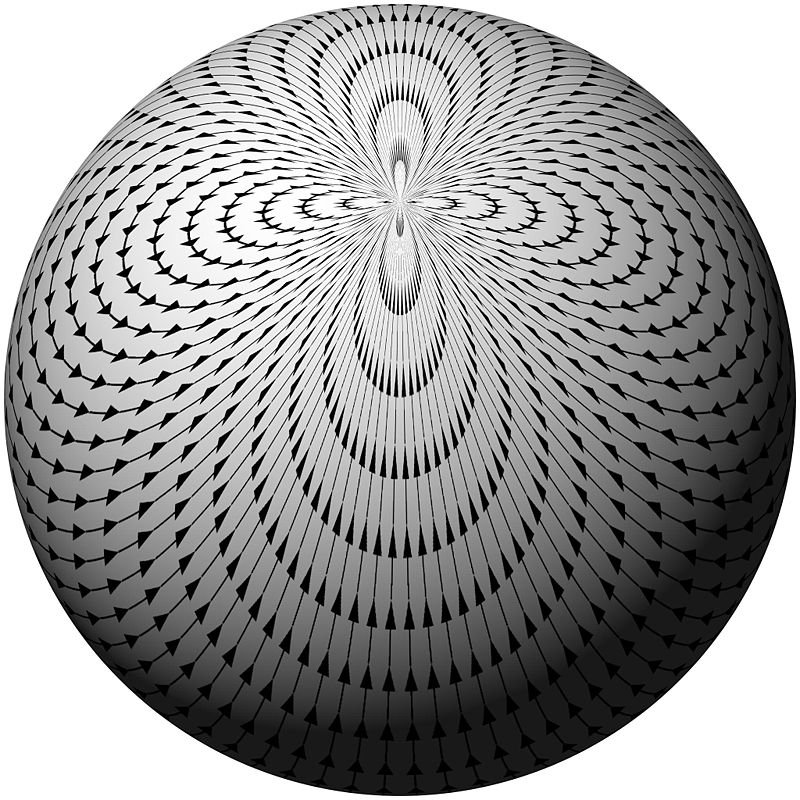
\includegraphics[width=0.4\textwidth]{Images/hairyball}
  \caption{An isolated singular point guaranteed by the Poincar\'e-Hopf
    theorem\footnotemark}
\end{figure}   
    \footnotetext{Image Courtesy of Wikipedia: RokerHRO - Own work, CC BY-SA 3.0,
    \url{https://commons.wikimedia.org/w/index.php?curid=8257798}}
\begin{theorem}[The Hairy Ball Theorem] You can't comb a hairy ball without
  a bald spot. Or, in more precise terms, let $f$ be a continuous function
  that assigns a vector in $\mathbb{R}^3$ to each point on $S^2$, such that
  $f(p)$ is tangent to $S^2$ at $p$. Then, there is at least one $p$ for
  such that $f(p)=0$.
\end{theorem}
\begin{proof}
  Assume, in order to find a contradiction, that $f(p)\neq 0$ for all $p$ on
  the 2-sphere. Then, there exists a vector field $v$ on $S^2$ such that $v$
  has no singular points. However, given the above theorem, this is
  a contradiction, as we know that there must exist two distinct isolated
  singular points on this vector field, thusly there can be no such vector
  field on the sphere or on any manifold topologically homeomorphic to the
  sphere.
\end{proof}
asdsadd

%%%%%%%% END OF INCLUSION %%%%%%%%%%%

%%%%%%%%% BIBLIOGRAPHY %%%%%%%%%%
\nocite{*}
\bibliographystyle{plain}
\bibliography{biblio.bib}
%%%%%%%% END BIBLIOGRAPHY %%%%%%%%
\printindex

\end{document}
